%%%%%%%%%%%%%%%%%%%%%%%%%%%%%%%%%%%%%%%%
% Classe do documento %
%%%%%%%%%%%%%%%%%%%%%%%%%%%%%%%%%%%%%%%%

% Nós usamos a classe "unb-cic".  Deixe apenas uma das linhas
% abaixo não-comentada, dependendo se você for do bacharelado ou
% da licenciatura.

\documentclass[bacharelado]{unb-cic}
%\documentclass[licenciatura]{unb-cic}



%%%%%%%%%%%%%%%%%%%%%%%%%%%%%%%%%%%%%%%%
% Pacotes importados
%%%%%%%%%%%%%%%%%%%%%%%%%%%%%%%%%%%%%%%%

\usepackage[brazil,american]{babel}
\usepackage[T1]{fontenc}
\usepackage{indentfirst}
\usepackage{natbib}
\usepackage{amsmath}
\usepackage{mathtools}
\usepackage{xcolor,graphicx,url}
\usepackage{subcaption}
\usepackage{url}
\usepackage[utf8]{inputenc}
\usepackage{float}


%%%%%%%%%%%%%%%%%%%%%%%%%%%%%%%%%%%%%%%%
% Caminho das imagens
%%%%%%%%%%%%%%%%%%%%%%%%%%%%%%%%%%%%%%%%%
\graphicspath{ {imagens/} }


%%%%%%%%%%%%%%%%%%%%%%%%%%%%%%%%%%%%%%%%
% Cores dos links
%%%%%%%%%%%%%%%%%%%%%%%%%%%%%%%%%%%%%%%%

% Veja o arquivos cores.tex se quiser ver que outras cores estão
% pré-definidas.  Utilizando o comando \hypersetup abaixo nós
% evitamos aquelas caixas vermelhas feias em volta dos links.

%%%%%%%%%%%%%%%%%%%%%%%%%%%%%%%%%%%%%%%%
% Cores do estilo Tango
%%%%%%%%%%%%%%%%%%%%%%%%%%%%%%%%%%%%%%%%

\definecolor{LightButter}{rgb}{0.98,0.91,0.31}
\definecolor{LightOrange}{rgb}{0.98,0.68,0.24}
\definecolor{LightChocolate}{rgb}{0.91,0.72,0.43}
\definecolor{LightChameleon}{rgb}{0.54,0.88,0.20}
\definecolor{LightSkyBlue}{rgb}{0.45,0.62,0.81}
\definecolor{LightPlum}{rgb}{0.68,0.50,0.66}
\definecolor{LightScarletRed}{rgb}{0.93,0.16,0.16}
\definecolor{Butter}{rgb}{0.93,0.86,0.25}
\definecolor{Orange}{rgb}{0.96,0.47,0.00}
\definecolor{Chocolate}{rgb}{0.75,0.49,0.07}
\definecolor{Chameleon}{rgb}{0.45,0.82,0.09}
\definecolor{SkyBlue}{rgb}{0.20,0.39,0.64}
\definecolor{Plum}{rgb}{0.46,0.31,0.48}
\definecolor{ScarletRed}{rgb}{0.80,0.00,0.00}
\definecolor{DarkButter}{rgb}{0.77,0.62,0.00}
\definecolor{DarkOrange}{rgb}{0.80,0.36,0.00}
\definecolor{DarkChocolate}{rgb}{0.56,0.35,0.01}
\definecolor{DarkChameleon}{rgb}{0.30,0.60,0.02}
\definecolor{DarkSkyBlue}{rgb}{0.12,0.29,0.53}
\definecolor{DarkPlum}{rgb}{0.36,0.21,0.40}
\definecolor{DarkScarletRed}{rgb}{0.64,0.00,0.00}
\definecolor{Aluminium1}{rgb}{0.93,0.93,0.92}
\definecolor{Aluminium2}{rgb}{0.82,0.84,0.81}
\definecolor{Aluminium3}{rgb}{0.73,0.74,0.71}
\definecolor{Aluminium4}{rgb}{0.53,0.54,0.52}
\definecolor{Aluminium5}{rgb}{0.33,0.34,0.32}
\definecolor{Aluminium6}{rgb}{0.18,0.20,0.21}

\hypersetup{
  colorlinks=true,
  linkcolor=DarkScarletRed,
  citecolor=DarkScarletRed,
  filecolor=DarkScarletRed,
  urlcolor= DarkScarletRed
}



%%%%%%%%%%%%%%%%%%%%%%%%%%%%%%%%%%%%%%%%
% Informações sobre a monografia
%%%%%%%%%%%%%%%%%%%%%%%%%%%%%%%%%%%%%%%%

\title{Detecção e monitoramento de vagas disponíveis em estacionamentos abertos através de processamento de imagens}

\orientador{\prof \dr Alexandre Zaghetto}{CIC/UnB}
%\coorientador[a]{\prof[a] \dr[a] Coorientadora}{MAT/UnB}
\coordenador{\prof \dr Rodrigo Bonifácio de Almeida}{CIC/UnB}
\diamesano{28}{Novembro}{2016}

\membrobanca{\prof \dr Flávio Barros Vidal}{CIC/UnB}
\membrobanca{MsC. Luiz Henrique Morais Aguiar}{CIC/UnB}

\autor{Vitor de Alencastro}{Lacerda}
\CDU{004.4}

\palavraschave{Estacionamento, Vagas livres, Processamento de Imagens, Redes Neurais, Fluxo Óptico, GLCM }
\keywords{Parking lots,Free Spaces, Image processing, Neural Networks, Optical Flow, GLCM}



%%%%%%%%%%%%%%%%%%%%%%%%%%%%%%%%%%%%%%%%
% Texto
%%%%%%%%%%%%%%%%%%%%%%%%%%%%%%%%%%%%%%%%


\begin{document}
  \maketitle
  \pretextual

  \begin{dedicatoria}
  Dedico a todos os outros motoristas frustrados que gostariam de perder menos tempo estacionando seus carros.
  \end{dedicatoria}

  \begin{agradecimentos}
  Agradeço a minha família e amigos pelo apoio durante toda a longa duração do curso e da elaboração deste trabalho e ao professor Alexandre Zaghetto pela orientação.
  \end{agradecimentos}

  \begin{resumo}
  Encontrar vagas livres em grandes estacionamentos muitas vezes é uma tarefa frustrante e que consome muito tempo. Soluções que ajudam um motorista a encontrar uma vaga mais rapidamente economizam tempo e dinheiro, além de servir como fator diferencial entre estabelecimentos comerciais. Este trabalho apresenta um programa que analisa a imagem de uma câmera que filma um estacionamento e determina a ocupação das vagas presentes na imagem através da detecção de movimento no vídeo e uma rede neural artificial. Uma solução como esta, que utiliza técnicas de processamento de imagens, tem custo de instalação e manutenção muito menor do que o uso de sensores individuais nas vagas, além de ser muito mais adequada para uso em grandes estacionamentos descobertos.
  \end{resumo}

  \selectlanguage{american}
  \begin{abstract}
  Finding free parking spaces in big parking lots is often a frustrating and time-consuming task. Solutions that help drivers find spaces faster save both time and money, and can help attract customers to commercial establishments. This work presents an approach that analyzes images from a camera filming a parking lot and determines parking space occupancy through movement detection and an artificial neural network. Solutions that use image processing techniques have much lower installation and maintenance costs than solutions that involve individual sensors. They are also more adequate for outdoor parking lots.
  \end{abstract}
  \selectlanguage{brazil}

  \tableofcontents
  \listoffigures
  \listoftables

  \textual
  \chapter{Introdução}\label{cap:intro}

			Atualmente, a frota de carros dos grandes centros urbanos fica cada vez maior. Esse aumento no número de veículos cria uma demanda por espaço de estacionamento, levando a construção de novos estacionamentos e uma dificuldade muito maior de se encontrar vagas disponíveis nos estacionamentos existentes nos estabelecimentos comerciais, áreas residenciais e centros urbanos.
			Dele
			De fato, todo ano, milhões de pessoas gastam milhares de horas rondando estacionamentos de supermercados, \textit{shoppings} e prédios comerciais em busca de uma vaga de estacionamento vazia. Procurar por uma vaga em um estacionamento grande e cheio é uma tarefa cansativa e desagradável. Muitas vezes vagas desocupadas não são encontradas por motoristas que preferem parar seu carro e esperar que uma vaga próxima seja liberada. Outras vezes possíveis clientes desistem de ir a um determinado estabelecimento pois sabem da dificuldade de estacionar que enfrentarão. Esse problema é comum principalmente em \textit{shopping centers} e grandes supermercados, que possuem seus próprios estacionamentos disponíveis para os clientes, mas que estão frequentemente muito cheios.
			
			Facilitar a tarefa da busca de vagas em estacionamentos de estabelecimentos como estes, é benéfico então não só para os clientes, mas também para os donos e gerentes desses estabelecimentos. Sendo assim, esse trabalho tem como objetivo criar um sistema que seja capaz de determinar a ocupação das vagas de um estacionamento descoberto e informar quantas vagas estão disponíveis e a sua localização aproximada para os motoristas através do processamento de imagens do estacionamento. Tal solução facilitaria a procura de vagas, diminuindo o tempo gasto trafegando por fileiras de vagas ocupadas.
			
			A solução apresentada utiliza redes neurais artificais combinadas com técnicas descritoras de textura e características de crominância para diferenciar imagens de carros de imagens de vagas desocupadas. Cada região que contém vagas na imagem obtida é dividida em diversas seções verticais. Cada seção será classificada entre vaga vazia ou veículo, de forma que o programa então é capaz de determinar quantas vagas estão ocupadas nessa região e, consequentemente, quantas estão vazias. Algumas soluções propostas em trabalhos correlatos serão apresentadas no Capítulo \ref{cap:trabalhos}.
			
			No Capítulo \ref{cap:fundament} serão apresentados alguns conceitos importantes para o entendimento da solução que será apresentada posteriormente. Serão detalhados o que é uma imagem, como funciona um vídeo e outros elementos teóricos importantes como espaços de cores e descritores de textura. O Capítulo \ref{cap:redes} apresenta uma fundamentação teórica de redes neurais artificiais. Esse assunto foi separado em um capítulo próprio por causa da grande quantidade de conteúdo e por sua importância especial neste trabalho.
			
			No Capítulo \ref{cap:solucao}, a solução proposta é apresentada. Nesta seção será detalhado o funcionamento do sistema criado, o fluxo de execução do programa e os elementos que permitem o funcionamento do sistema.
			
			Em seguida, o Capítulo \ref{cap:results} apresentará resultados obtidos em testes que comparavam o sistema a observadores humanos, seguidos de observações sobre os resultados do programa. Esse capítulo também apresenta os detalhes da rede neural artificial utilizada.
			
			O Capítulo \ref{cap:conclusao} possui comentários sobre a taxa de sucesso do trabalho, suas fragilidades, sua adequação para uso no estado atual e se o objetivo desejado foi alcançado. O capítulo finaliza o trabalho com um comentário sobre possíveis trabalhos futuros para a evolução do sistema.
			
			









	\chapter{Fundamentação Teórica}\label{cap:fundament}



Esse capítulo tem como objetivo apresentar conceitos que facilitarão o entendimento do conteúdo do capítulo \ref{cap:solucao}, detalhando técnicas e conceitos utilizados na execução do trabalho através de exemplos e imagens. Serão apresentados conceitos relacionados ao processamento de imagens estáticas, seguidos de uma discussão breve sobre técnias aplicadas em vídeos. O conteúdo deste capítulo continua no cápitulo \ref{cap:redes} que apresenta conceitos de redes neurais e classificação de padrões. 

\section{Processamento de Imagens}\label{sec:processamento}

\subsection{Imagens em nível de cinza}

Para que um computador seja capaz de operar sobre uma imagem, é preciso que seja utilizado um modelo de representação que traduza o que os nossos sentidos conseguem perceber em informações que podem ser interpretadas por uma máquina que não é dotada de visão. A forma mais simples de se representar uma imagem são as imagens em nível de cinza. Podemos definir imagens como uma função \textit{f{(x,y)}} onde x e y são coordenadas espaciais e o valor de  \textit{f{(x,y)}} é a luminosidade, ou nível de cinza, da imagem naquele ponto. Quando esses valores são todos discretos, chamamos essa imagem de uma imagem digital.\cite{gonzalez2009digital} Cada elemento individual dessa imagem, cada valor em cada coordenada, pode ser chamado de um \textit{picture element} ou mais comumente \textit{pixel}. Em imagens digitais em nível de cinza, cada \textit{pixel} possui 1 \textit{bit} de informação, ou seja, pode assumir valores entre 0 e 255, onde o valor 0 representa o preto e 255 representa o branco. 

Uma imagem então, pode ser interpretada por um programa de computador como uma matriz $MxN$ de elementos de 1 \textit{bit}, onde M é a largura da imagem e N é a sua altura. Cada elemento $p_{i,j}$ da matriz possui a informação de luminosidade do pixel correspondente e o computador é capaz de exibir e interpretar esses valores apropriadamente. A figura \ref{fig:NivelCinza} exemplifica esse processo.

\begin{figure}
 \centering
\begin{subfigure}{.5\textwidth}
  \centering
  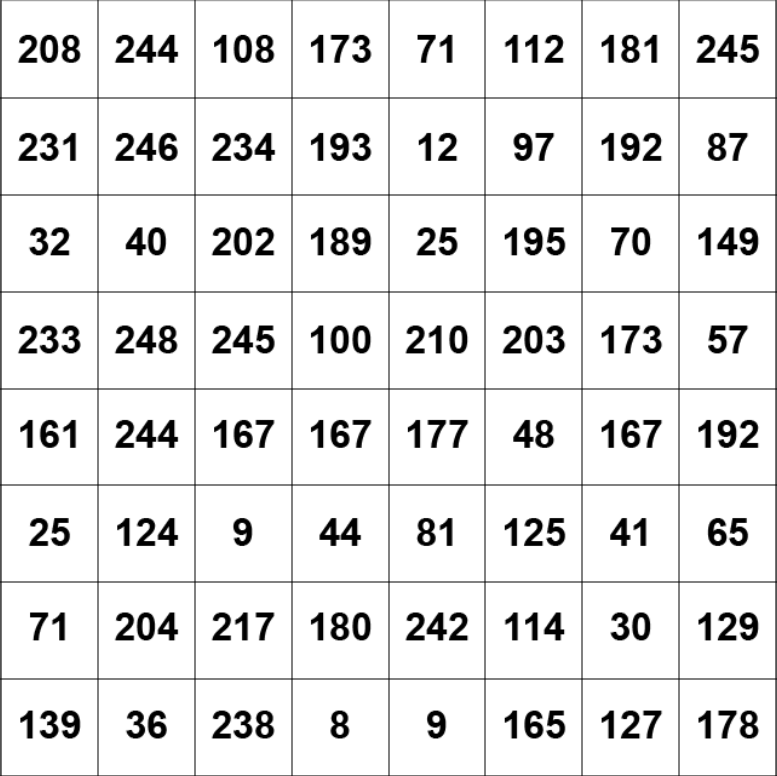
\includegraphics[width=.5\linewidth]{MatrizNivelCinza}
  \caption{}
  \label{exemplo:sfig1}
  \centering
\end{subfigure}%
\begin{subfigure}{.5\textwidth}
  \centering
  
\includegraphics[width=.5\linewidth]{ExemploNivelCinza}
  \caption{}
  \label{exemplo:sfig2}
  \centering
\end{subfigure}
\caption{(a) Uma matriz com níveis de cinza e (b) a imagem correspondente}
\label{fig:NivelCinza}
\centering
\end{figure}


\subsection{Espaços de cores}

Para que um sistema de processamento de imagens possa interpretar e processar cores, é preciso criar modelos apropriados para representá-las. Chamamos os modelos de representação das cores em uma imagem um espaços de cor. Existem diversos espaços de cor, cada um importante para a realização de tarefas e necessidades diferentes. Para a compreensão deste trabalho, é necessário, porém, entender apenas dois: o espaço RGB e o espaço YCbCr.

\subsection{O espaço RGB}


RGB é um acrônimo para \textit{Red, Green, Blue}, vermelho, verde e azul em inglês. Pesquisas mostram que um grande gama de cores pode ser formado através de combinações aditivas das cores vermelho, verde e azul. Essas cores são consideradas então cores primárias aditivas.\cite{IBGE2000introducao}. Nesse modelo, a cor de um \textit{pixel} de uma imagem é representada através de três coeficientes que definem a influência de cada cor primária na combinação. Uma imagem no modelo RGB é então representada por três matrizes de níveis de cinza de dimensões iguais, chamadas canais, onde cada valor representado na matriz, representa o valor do coeficiente da cor correspondente na imagem final. Isto é, a imagem pode ser representada por uma matriz $MxNx3$ onde a cor final $C_{i,j}$ de cada \textit{pixel} da imagem é definida pela equação \ref{eq:corRGB}. A imagem \ref{fig:Espacos:sub:RGB} mostra os canais de uma imagem RGB separadamente.

Esse espaço de cor é o mais comumente usado para representar imagens que vemos no cotidiano, uma vez que é semelhante a visão humana e portanto é utilizado pelos dispositivos multimídia mais comuns.
	
	\begin{equation}
			C_{i,j} = p_{i,j,1} . R + p_{i,j,2} . G + p_{i,j,3} . B ,  (1<i<M, 1<j<N)
	\label{eq:corRGB}
	\end{equation}

\subsection{Espaço YCbCr}\label{sect:sub:ycbcr}

Assim como o espaço de cor RGB, o espaço YCbCr também representa uma imagem através de três matrizes, porém, seus canais contém informações diferentes do modelo RGB. Esse modelo é muito utilizado para o armazenamento de vídeos, uma vez que o modelo tira vantagem de alguns aspectos da visão humana para poder armazenar menos dados, sem perda significativa de informação visual. Por exemplo, humanos são mais sensíveis à detalhes e variações em níveis de cinza do que detalhes em imagens coloridas. Além disso, o olho humano é mais sensível ao verde do que qualquer outra cor\cite{colorSpacesDigitalVideo}. Com esse conhecimento, o espaço YCbCr representa as cores de uma imagem através de sua luminosidade(Y) e os valores de crominância azul(Cb) e crominância vermelha(Cr). Cb e Cr são sinais de diferença de cor e são definidos pela subtração do valor de luminosidade do canal azul e vermelho da imagem, respectivamente. A luminosidade é definida pela equação \ref{eq:Y}\cite{LivroVideoDigital} que reflete a sensibilidade maior a cor verde da visão humana.

Na figura \ref{fig:Espacos:sub:YCbCr} estão exemplificados os canais de uma imagem no espaço YCbCr.

\begin{equation}
	Y = 0,299.R + 0,587.G + 0,114.B
\label{eq:Y}
\end{equation}


\begin{figure}
 \centering
\begin{subfigure}{.5\textwidth}
  \centering
  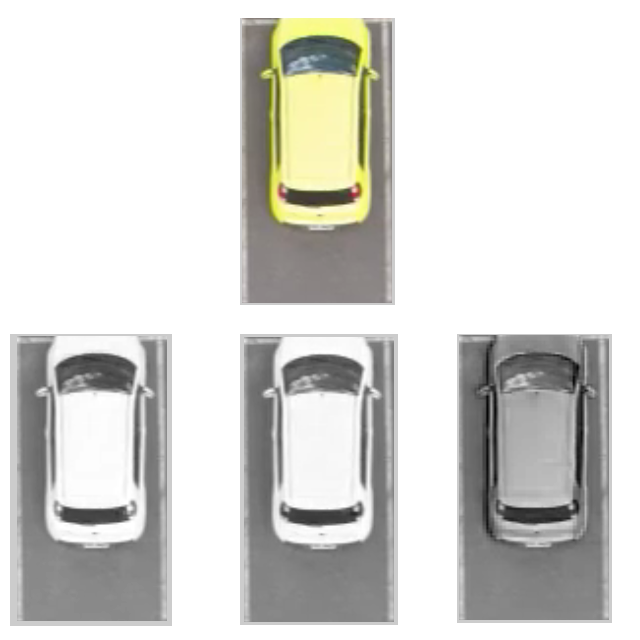
\includegraphics[width=.8\linewidth]{exemploRGBFinal}
	\caption{}
	\label{fig:Espacos:sub:RGB}
	\centering
\end{subfigure}\
\begin{subfigure}{.5\textwidth}
  \centering
  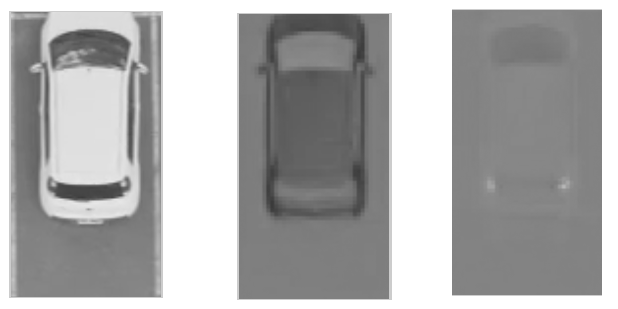
\includegraphics[width=.8\linewidth]{exemploYCbCrFinal}
	\caption{}
	\label{fig:Espacos:sub:YCbCr}
	\centering
\end{subfigure}
\caption{(a) Uma imagem e cada um de seus canais RGB ordenados da esquerda para a direita e (b) os canais YCbCr da imagem ordenados da esquerda para a direita.}
\label{fig:Espacos}
\centering
\end{figure}

\subsection{Descritores de textura}\label{sec:descritores}

Descritores de textura são algoritmos que procuram fazer o que o olho humano faz com facilidade: distinguir tipos diferentes de objetos apenas por algumas de suas características visuais. Estes algoritmos são utilizados quando a abordagem de processamento \textit{pixel-a-pixel} se mostra insuficiente. Eles observam e analisam características pertinentes a imagem inteira e são capazes de identificar diferenças mais sutis entre imagens diferentes. Existem diversas técnicas de descrição de textura que são utilizadas com sucesso em aplicações de processamento de imagem. Para esse trabalho, a técnica escolhida foi a conhecida como GLCM(\textit{gray-level co-ocurrence matrix}) descrita na seção \ref{sec:GLCM}, por ter execução rápida e ser invariante quanto a escala de cinza.

\subsection{GLCM}\label{sec:GLCM}

GLCM, ou matriz de co-ocorrência de nível de cinza, é uma técnica de descrição de textura que visa extrair medidas estatíticas da imagem sendo analisada. Para tanto, é criada uma matriz quadrada de tamanho $MxM$ onde M é a quantidade de níveis de cinza possíveis na imagem em questão. Essa matriz armazena a probabilidade de dois \textit{pixels} se relacionarem através de uma certa relação espacial\cite{GLCM}. 

Para esse trabalho, a relação observada é a da vizinhança entre dois \textit{pixels}, sempre analisando o valor a direita de um determinado \textit{pixel} da imagem. Os 255 valores de intensidade possíveis são divididos em 8 níveis. Cada elemento $P_{i,j}$ na GLCM $G$ conta a quantidade de vezes que um \textit{pixel} com valor de intensidade  $j$ apareceu à direita de um \textit{pixel} com valor $i$. A figura \ref{fig:GLCM} exemplifica a criação da GLCM a partir de uma imagem com 8 níveis possíveis.

\begin{figure}
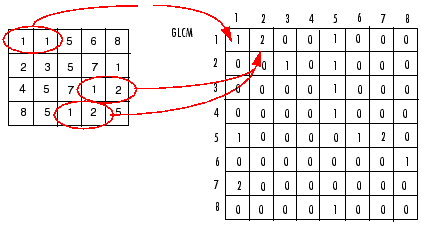
\includegraphics[width=8cm]{GLCM} 
\centering
\caption{Exemplo da elaboração da GLCM. Extraída de https://www.mathworks.com/help/images/ref/graycomatrix.html}
\label{fig:GLCM}
\centering
\end{figure}

Uma vez criada a matriz de co-ocorrência, diversas medidas podem ser extraídas. Para esse trabalho são extraídas as quatro características definidas abaixo. Nas equações apresentadas $P_{(i,j)}$ representa o valor do elemento na posição $(i,j)$ da GLCM, $\mu_i$ e $\mu_j$ representam a média dos valores de $i$ e $j$ respectivamente e $\sigma_i$ e $\sigma_j$ os desvios padrão destes valores.

\begin{itemize}

\item \textbf{Contraste}: mede o contraste entre um \textit{pixel} e seu vizinho na imagem. Deve ser 0 para uma imagem completamente homogênea. Definido por:
	\begin{equation}
		C = \sum_{i,j} (i-j)^{2}P_{(i,j)}
	\label{eq:Contraste}
	\end{equation}
	
\item \textbf{Correlação}: mede a taxa de correlação de um \textit{pixel} e seu vizinho na imagem inteira. Definida por:
	\begin{equation}
		Co = \sum_{i,j} \frac{(i - \mu_i)(j - \mu_j)P_{(i,j)}}{\sigma_i\sigma_j}
	\label{eq:Correlacao}
	\end{equation}
	
\item \textbf{Energia}: soma do quadrado dos elementos da imagem. Definida por:
	\begin{equation}
		E = \sum_{i,j} P_{(i,j)}^{2}
		\label{eq:Energia}
	\end{equation}
	
\item \textbf{Homogeneidade}: mede a proximidade da distribuição dos elementos à diagonal da matriz. Definida por:
	\begin{equation}
		H = \sum_{i,j} \frac{P_{(i,j)}}{1+|i-j|}
		\label{eq:Homo}
	\end{equation}

\end{itemize}


\section{Vídeos}\label{sec:video}


Quando observamos uma cena no mundo real, ela raramente é estática. Com o passar do tempo, os objetos presentes nela se movem continuamente pelo espaço, criando infinitas imagens diferentes em nossas retinas. Podemos simular essa sensação de movimento na nossa visão através da exibição rápida de imagens que contém valores discretos. Esse é o conceito de um vídeo digital. Um vídeo digital é formado através da amostragem de imagens	em três eixos: horizontal, vertical e temporal\cite{LivroVideoDigital}. A cada intervalo fixo de tempo, uma imagem representada por uma matriz bidimensional de valores de intensidade luminosa e cor é amostrada. Cada uma dessas imagens, ou quadros, representa o estado da cena naquele momento no tempo.

\subsection{Fluxo Óptico}\label{sec:fluxooptico}

O movimento é um dos elementos principais para a extração de informações de um vídeo. O fluxo óptico, ou \textit{optical flow}, é uma das técnicas para a estimativa de movimento em vídeos digitais. A técnica consiste em medir a projeção 2D no plano da imagem de um movimento real 3D\cite{mota2011tensor}. Essa projeção 2D mede a velocidade de cada \textit{pixel} da imagem. Esses vetores de velocidade da imagem podem ser utilizados para a realização de diversas tarefas. Por exemplo, é possível extrair a magnitude dos vetores e criar uma nova imagem, aonde os valores de intensidade representam o movimento realizado pelo \textit{pixel}. Nesse trabalho, essa técnica é utilizada para a segmentação de objetos em movimento contra um fundo estático, detalhada no capítulo \ref{cap:solucao}. A figura \ref{fig:fluxo} mostra os vetores de movimento calculados e uma imagem em níveis de cinza que representa as magnitudes das velocidades de cada pixel.

\begin{figure}
 \centering
\begin{subfigure}{.5\textwidth}
  \centering
  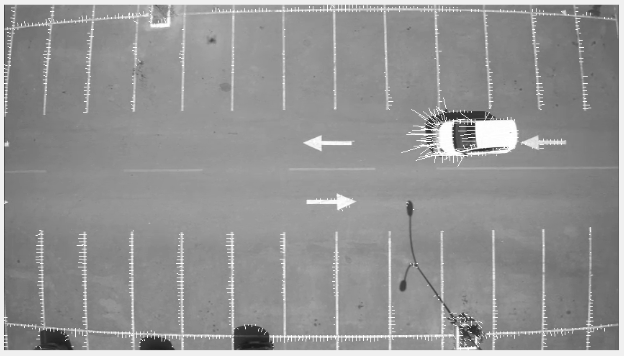
\includegraphics[width=.8\linewidth]{velocidadevetores}
	\caption{}
	\label{fig:fluxo:sub:vetores}
	\centering
\end{subfigure}\
\begin{subfigure}{.5\textwidth}
  \centering
  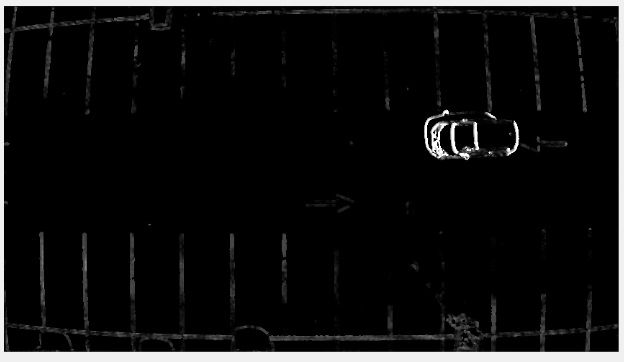
\includegraphics[width=.8\linewidth]{velocidademagnitude}
	\caption{}
	\label{fig:fluxo:sub:magnitude}
	\centering
\end{subfigure}
\caption{(a) Representação dos vetores de velocidade estimado pelo fluxo óptico. (b) Imagem em níveis de cinza onde a intensidade do \textit{pixel} representa a magnitude do seu vetor de velocidade.}
\label{fig:fluxo}
\centering
\end{figure}

Para calcular o fluxo óptico, começamos assumindo que no intervalo entre dois quadros a intensidade de cada \textit{pixel} não muda de forma significativa. Chamamos então a intensidade de cada \textit{pixel} na posição (x,y) em um determinado momento $t$ de $I(x,y,t)$ e portanto, podemos dizer que: 

\begin{equation}
	I(x,y,t) = I(x+dx, y+dy, t+dt)
\label{eq:fluxo1}
\end{equation} 

onde $dx$ e $dy$ são o deslocamento que o \textit{pixel} no intervalo $dt$ entre dois quadros.

Queremos então encontrar a velocidade $v =(\frac{dx}{dt},\frac{dy}{dt})$ do \textit{pixel}. Usando a expansão por série de Taylor e manipulações matemáticas na equação \ref{eq:fluxo1}, obtemos a equação \ref{eq:fluxo2}\cite{faria1992fluxo}.

\begin{equation}
	\nabla Iv + I_t = 0
\label{eq:fluxo2}
\end{equation}

onde $\nabla I$ é o gradiente da função intensidade. Essa equação descreve o chamado problema de Restrição do Fluxo Óptico\cite{mota2011tensor}. Porém, há um problema na equação. A partir dela só é possível obter um dos componentes da velocidade. A solução completa da velocidade depende de um cálculo na vizinhança de cada ponto. Diversos métodos foram criados para a fazer a estimativa da velocidade, com propriedades diversas. Para esse trabalho foi escolhido o método desenvolvido por Lucas e Kanade, detalhado em \cite{faria1992fluxo}\cite{mota2011tensor} e \cite{bruhn2005lucas}. Este método se utiliza de características de uma vizinhança local e visa minimizar o erro de mínimos quadrados. Foi escolhido por ser resistente a ruído e ter mostrado um resultado mais adequado para as exigências do trabalho.

O capítulo \ref{cap:redes} continua a apresentação de conceitos importantes para o entendimento do trabalho, mas tem foco exclusivo em redes neurais artificiais. 







	%\chapter{Redes Neurais Artificiais} \label{cap:redes}

Comparado com os computadores mais avançados que existem hoje, o cérebro humano ainda se mostra muito mais poderoso e eficaz do que as máquinas. O cérebro é capaz de processar informação a uma velocidade muito maior do qualquer computador convencional e realiza com facilidade tarefas como o reconhecimento de padrões e classificação de objetos, enquanto algoritmos tradicionais falham. 

Redes neurais artificiais foram criadas com inspiração no funcionamento e na estrutura do cérebro, como uma alternativa poderosa para resolver problemas que as arquiteturas tradicionais não eram capazes de resolver eficientemente. Essas redes emulam a estrutura cerebral natural, se utilizando de elementos distintos de processamento (neurônios) que se comunicam para realizar a tarefa desejada. 

Simon Haykin\cite{Haykin} define uma rede neural como "...um processador distribuído massivamente paralelo composto por unidades simples de processamento, que possui uma propensidade natural a armazenar conhecimento experimental e torná-lo disponível para uso."

As redes neurais artificiais são utilizadas para resolver problemas como ajuste de funções, classificação de objetos e reconhecimento de padrões. Nesse capítulo, serão explicados conceitos importantes para o entendimento das redes artificiais, começando pelo seu elemento mais básico, o neurônio.

\section{Neurônios}

O neurônio é a estrutura básica do sistema nervoso central. É uma célula composta principalmente de três partes distintas: o corpo celular, os dendritos e o axônio. O corpo celular é a estrutra central do célula aonde está contido o núcleo do neurônio e são executados as suas funções vitais. Os dendritos são prolongamentos do corpo celular responsáveis por receber sinais e o axônio é uma extensão maior do corpo celular, responsável por enviar sinais a outros neurônios. Dois neurônios interagem em apenas  pontos de contato chamados sinapses. Nessas sinapses o axônio de um neurônio envia sinais para os dendritos de um segundo neurônio. A figura \ref{fig:neuronio} ilustra a estrutura básica dos neurônios.

\begin{figure}
\centering
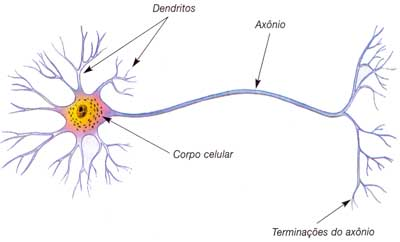
\includegraphics[width=.6\textwidth]{neuronio}
\label{fig:neuronio}
\caption{A estrutura básica de um neurônio humano}
\end{figure}

O neurônio artificial também possui três estruturas básicas semelhantes àquelas do neurônio natural. Seus três elementos básicos são: as entradas(análogas aos dendritos), a sáida(análoga ao axônio) e um núcleo de processamento. 

O neurônio pode ter uma ou mais conexões de entrada caracterizadas por um peso $wi$ e que recebe um valor $xi$. No núcleo do neurônio artificial há um somador que calcula o valor $u$ agregado das entradas, ponderadas pelo peso correspondente. O resultado dessa soma ponderada é então deslocado de um valor escalar e em seguida submetido a uma função chamada de função de ativação, que determina a saída final do neurônio. Em suma podemos descrever a saída de um neurônio $n$ que possui $i$ entradas através das seguintes equações:

\begin{equation}
 u_n = \sum_{j=1}^i x_jw_j
\end{equation}

\begin{equation}
s(n) = f(u_n + b)
\end{equation}

Aonde $u_n$ é o valor agregado das entradas, $x_j$ é a j-ésima entrada e $w_j$ o peso da conexão associada, $s(n)$ é a saída do neurônio, $f$ é a função de ativação e $b$ o deslocamento, ou $bias$ do neurônio $n$. A figura \ref{fig:neuroartificial} ilustra a estrutura básica de um neurônio artificial.

%imagem do neurônio artifical

Claramente, a função de ativação do neurônio é o grande fator que define o seu comportamento e consequentemente sua funcionalidade. Existem dois tipos básicos de funções de ativação\cite{Haykin}: a função degrau e a função sigmóide.

O neurônio mais simples possível tem sua saída regida por uma função degrau e saída binária. Isto é, se o valor agregado $u$ de suas entradas for maior que um determinado limiar, a sua saída será 1 e a saída será 0 caso contrário. Apesar de ser capaz de resolver alguns problemas, esse tipo de neurônio tem algumas desvantagens. Por vezes, alterações sutis podem representar a diferença entre os dois valores possíveis da sáida. Além disso, um alcance limitado de valores na saída prejudica o treinamento.

A escolha mais comum de de função de ativação para a construção de redes neurais é a família de funções sigmóides. Essas funções, que tem um gráfico com formato de \textit{S}, assumem valores contínuos entre 0 e 1, o que faz com que alterações sutis na entrada representem alterações mais sutis na saída, aumentando a qualidade da informação gerada pelo neurônio. A mais comum das funções sigmóides utilizadas é a função logística, definida pela equação \ref{eq:logistica}, onde $a$ é uma constante que mede a declividade da curva.

\begin{equation}
	f(u) = \frac{1}{1 + \exp{-au}}
\label{eq:logistica}
\end{equation}

Um dos motivos que tornou a função logística uma escolha popular para os neurônios artificiais foi a sua derivação simples, uma vez que algoritmos de treinamento muitas vezes usam a derivada da função de ativação\cite{Kosabov}.

É interessante reparar que quando $a$ se aproxima do infinito, a função logística se comporta da mesma forma que a função degrau.

\begin{figure}
 \centering
\begin{subfigure}{.5\textwidth}
  \centering
  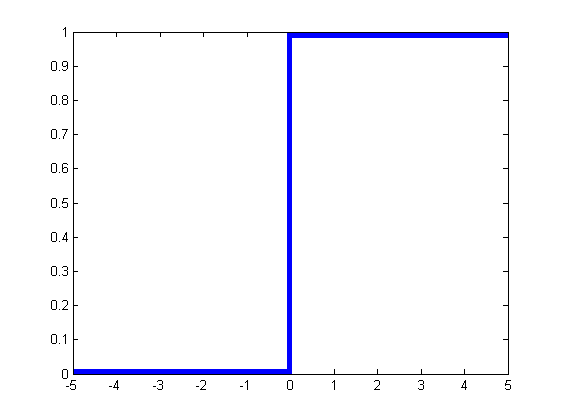
\includegraphics[width=.8\linewidth]{degrau}
	\caption{}
	\label{fig:ativacao:sub:degrau}
\end{subfigure}\
\begin{subfigure}{.5\textwidth}
  \centering
  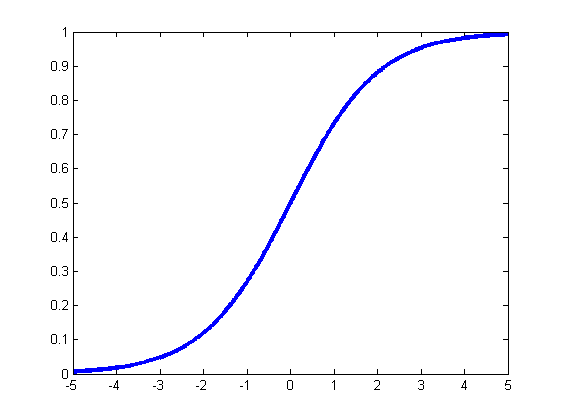
\includegraphics[width=.8\linewidth]{logistica}
	\caption{}
	\label{fig:ativacao:sub:logistica}
\end{subfigure}
\caption{(a) Gráfico da função degrau com limiar 0. (b) Gráfico da função logística com a = 1}
\label{fig:ativacao}
\end{figure}




\section{Redes Neurais Feed-Forward}

Apesar de neurônios serem capazes de resolver alguns problemas sozinhos, o verdadeiro poder das redes neurais vem da interconexão entre os neurônios de forma a criar ligações semelhantes às sinapses dos neurônios naturais.

Existem várias arquiteturas para a formação destas redes de neurônios, porém neste trabalho a discussão será limitada àquela utilizada na implementação do programa: as chamadas redes neurais \textit{feed-forward}.

São necessárias ao menos três camadas para a construção da rede neste modelo: a primeira camada, chamada de camada de entrada, uma ou mais camadas intermediárias(ou ocultas) e a camada de saída. O papel das camadas ocultas é intermediar entre as entradas externas e a saída da rede, de forma a possibilitar que a rede extraia dados estatíticos mais significativos da sua entrada.  Uma camada é composta de um número de neurônios que agem de forma paralela. Cada neurônio de uma camada que não é a de saída está conectado apenas ao neurônios da camada seguinte, de forma que não há comunicação entre uma camada e camadas anteriores a ela. Isto é, a informação flui na rede apenas no sentido entrada-saída, como ilustrado na figura \ref{fig:feedfoward}.

\begin{figure}
\centering
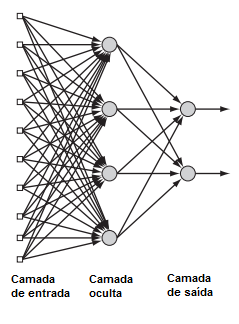
\includegraphics[width=.6\textwidth]{feedforward}
\label{fig:feedfoward}
\caption{A arquitetura feed-forward. Cada neurônio se comunica com os neurônios da camada seguinte até que a saída final seja produzida. Adaptada de \cite{Haykin}}
\end{figure}

O vetor de entrada da rede é alimentado aos neurônios da primeira camada, cuja saída serve de entrada para a segunda camada e assim por diante, até que a última camada seja alimentada pela saída da camada anterior e produza a saída final da rede. 

\section{Treinamento}

Para que uma rede neural artificical possa ser utilizada, ela precisa antes aprender a realizar a tarefa para a qual foi criada. Para isso a rede precisa ter duas abilidades importantes: de aprendizado e de generalização. Aprendizado é a capacidade da rede de aproximar o comportamento das entradas fornecidas durante o treinamento, enquanto generalização é a sua capacidade de prever e operar sobre dados além do conjunto com a qual foi treinada\cite{ZhangNNSurvey}.

É necessário então que a rede passe por um processo de treinamento, onde os valores dos pesos $wi$ e os deslocamentos $b$ de cada neurônio são definidos de forma que o funcionamento da rede seja ótimo para a tarefa que se deseja realizar. Para realizar o treinamento de uma rede, o primeiro passo é definir 3 conjuntos distintos de entradas:

\begin{itemize}
	\item \textbf{Conjunto de testes:} A rede é submetida às entradas deste conjunto para que seja feita a calibração dos valores da matriz de pesos $W$ e do vetor de deslocamentos $B$.
	
	\item \textbf{Conjunto de validação:} Após uma etapa de treinamento, a rede computa os dados deste conjunto de entradas para validar os valores da matriz $W$ e do vetor $B$ escolhidos até então.
	
	\item \textbf{Conjunto de testes:} Por fim, após o treinamento, a rede é submetida aos dados deste conjunto, a fim de verificar o seu funcionamento correto.
\end{itemize}

Isto é, a cada ciclo de treinamento, a rede ajusta os seus pesos e deslocamentos de acordo com o conjunto de treinamento, e em seguida processa os dados do conjunto de validação. Se for determinado que a rede teve sucesso no processo de validação, ela fica pronta pra passar pelo conjunto de testes, aonde as sua capacidade de generalização é testada. A matriz $W$ de pesos gerada durante este processo é uma forma de representação do "conhecimento" da rede. Assim, o aprendizado não é uma característica de cada neurônio, mas sim um processo que ocorre na rede inteira como resultado do treinamento\cite{Kozabov}.

Existem duas principais maneiras de se executar o treinamento de uma rede.

\begin{itemize}
	\item \textbf{Treinamento supervisionado:} Neste paradigma os conjunto de treinamento e de validação consistem em um grupo de vetores de entrada $x$ e um gabarito de vetores de saída desejado $y$. O treinamento acontece até que o vetor de saída da rede para uma determinada entrada $x_i$ seja suficientemente próximo do vetor gabarito $y_i$ correspondete.
	
	
	\item \textbf{Treinamento não-supervisionado:} Neste paradigma a rede apenas recebe um conjunto $x$ de entradas e aprende características intrínsicas do dados apresentados a ela.
	
\end{itemize}

Uma vez definido o paradigma de treinamento, é necessário definir uma técnica para a análise do erro e alteração dos valores da matriz de pesos $W$ e do vetor $B$ de deslocamentos. Uma das técnicas mais utilizadas é a chamada de \textit{backpropagation}\cite{DeepLearning, ZhangNNSurvey}. A técnica consiste de uma análise do erro apresentado na saída da rede, que então é utilizada para se percorrer a rede no sentido contrário dos dados modificando os valores de $W$ e $B$ de forma a diminuir o erro na próxima iteração. Essa técnica é muito utilizada para sistemas de treinamento supervisionado, onde o erro é avaliado através de uma comparação da saída da rede com o gabarito fornecido. Uma vez que a os valores de $W$ e $B$ param de mudar, diz-se que a rede atingiu um estado de convergência\cite{Kozabov} e o treinamento finaliza.


\section{Classificação de padrões}

	%\chapter{Trabalhos Correlatos} \label{cap:trabalhos}

Nesse capítulo serão expostas soluções para o problema apresentado no capítulo \ref{cap:intro}, acompanhadas de uma discussão sobre vantagens e desvantagens, e as razões pela escolha da solução proposta no capítulo \ref{cap:solucao}.

Podemos separar os métodos de detecção de vagas em duas grandes categorias: métodos intrusivos e não-intrusivos. Métodos intrusivos são caracterizados por exigirem instalações mais complexas, envolvendo a inserção de equipamento no asfalto do estacionamento ou em um estrutura de concreto. Os métodos não intrusivos normalmente se utilizam de equipamentos externos, que não exigem obras para a sua instalação.

Um exemplo comum de método itrusivo é o uso de sensores individuais em cada vaga do estacionamento. Diversos tipos de sensores podem ser utilizados, cada um com vantagens e desvantagens próprias \cite{idris09}. Sensores infravermelhos versáteis e de simples instalação, mas podem ser afetados por condições ambientais. Tubos pneumáticos e sensores de peso sob o asfalto têm alta cofiabilidade, mas exigem grandes obras para a instalação. 

Alguns tipos de sensores podem ser instalados de forma não intrusiva. Esses sensores podem ser afixados no teto ou em uma estrutura próxima a vaga. Sensores ultrassônicos por exemplo, pertencem a essa categoria. Eles transmitem ondas sonoras de baixa frequência e usam a energia refletida para determinar a ocupação das vagas \cite{kianpisheh2012smart}.

Intrusivos ou não, os métodos de detecção que utilizam sensores compartilham duas desvantagens: é necessário a instalação do sensor em cada uma das vagas, aumentando o custo do sistema e diminuindo sua escalabilidade, e eles não são adequados para estacionamentos descobertos, onde é impossível instalar sensores no teto e obras no asfalto rodoviário podem danificá-lo permanentemente \cite{idris09}.

Uma solução que se mostrou adequada para os estacionamentos descobertos foi o uso de \textit{softwares} de visão computacional, que analisam imagens de câmeras de vídeo para determinar a ocupação das vagas do estacionamento. Essa opção tem um custo baixo e exige apenas que sejam instaladas câmeras em pontos estratégicos do estacionamento. Uma vez que as câmeras foram instaladas e as imagens estão sendo capturadas, resta que seja executado um programa que as analise.

Para a escolha da abordagem para este trabalhos foram escolhidos os seguintes critérios principais:

\begin{itemize}
	
	\item O sistema deve poder ser instalado e começar sua execução em um estacionamento em qualquer estado, sem a necessidade de iniciar com todas as vagas descocupadas, possibilitando uma instalação a qualquer momento, sem interrupção das operações do estacionamento.
	\item O sistema deve necessitar de interação humana mínima, se limitando apenas uma rápida calibração no início de sua execução a fim de evitar erro humano.
	\item O sistema deve ser capaz de identificar a posição das vagas do estacionamento após um certo tempo de execução, e não através de entrada manual, para compensar por erros na calibração.
	\item O sistema deve, além de determinar o número de vagas livres no estacionamento, ser capaz de indicar a posição aproximada de tais vagas de forma a facilitar ainda mais a busca por uma vaga desocupada.
	
\end{itemize}

Em \cite{delibaltov2013parking}, Delibaltov \textit{et al} descrevem um método de detecção que estima um volume tridimensional para cada vaga marcada na imagem e depois se utiliza de redes neurais para determinar \textit{pixels} da imagem pertencentes a veículos. Em seguida a sistema computa a probabilidade de que uma certa vaga esteja ocupada baseado em uma função de probabilidade e os \textit{pixels} de veículo na região de interesse de cada vaga. Esse método se mostra preciso e eficaz, mas exige que o estacionamento esteja vazio e que cada vaga seja marcada individualmente no momento de execução, de forma que ele não é capaz de mapear as vagas do estacionamento ou detectar veículos estacionados irregularmente.

Bong \cite{bong2008integrated} propõe um sistema que se utiliza de subtração de imagens e o uso de detecção automática de coordenadas aproximadas das vagas para resolver este problema. Porém esse sistema exige que seja armazenada uma imagem do estacionamento completamente vazio, além de que seja criada uma imagem que marca cada vaga para o processo de inicialização do sistema.

Um sistema que se utiliza de uma técnica de classificação de histogramas de crominância em áreas de interesse e um algoritmo de que encontra pontos com \textit{features} relevantes foi proposto em \cite{true2007vacant}. Esse sistema tem a vantagem de ser relativamente invariante quanto a iluminação da imagem, por utilizar os canais de crominância para a análise. Também é bastante capaz de resolver o problema de oclusão de veículos atrás de outros na imagem de câmeras com uma angulação maior.

A solução proposta neste trabalho procura compensar alguns dos problemas presentes nos trabalhos mencionados, enquanto apresenta uma nova abordagem a ser considerada e aprimorada por trabalhos futuros.


	\chapter{Solução Proposta}\label{cap:solucao}









	\chapter{Resultados Experimentais}\label{cap:results}

\section{Aquisição de dados}

Para os experimentos realizados neste trabalho foi capturado um conjunto de vídeos no estacionamento do pavilhão João Calmon na Universidade de Brasília. Foram feitas duas seções de filmagens contínua, aonde três veículos se deslocavam pelo estacionamento e ocupavam vagas escolhidas arbitrariamente. O primeiro vídeo capturado foi utilizado para o treinamento da rede. O segundo vídeo foi dividido em oito vídeos de menor duração sobre os quais foram realizados os testes.

As filmagens foram realizadas por um drone modelo \textit{Yuneec Typhoon Q500+}\ref{fig:drone}. O drone foi controlado para que pairasse no ar em uma altura semelhante a de um poste de luz, a fim de capturar imagens de forma mais próxima possível de uma câmera de vídeo instalada em um poste de luz.

\begin{figure}
\centering
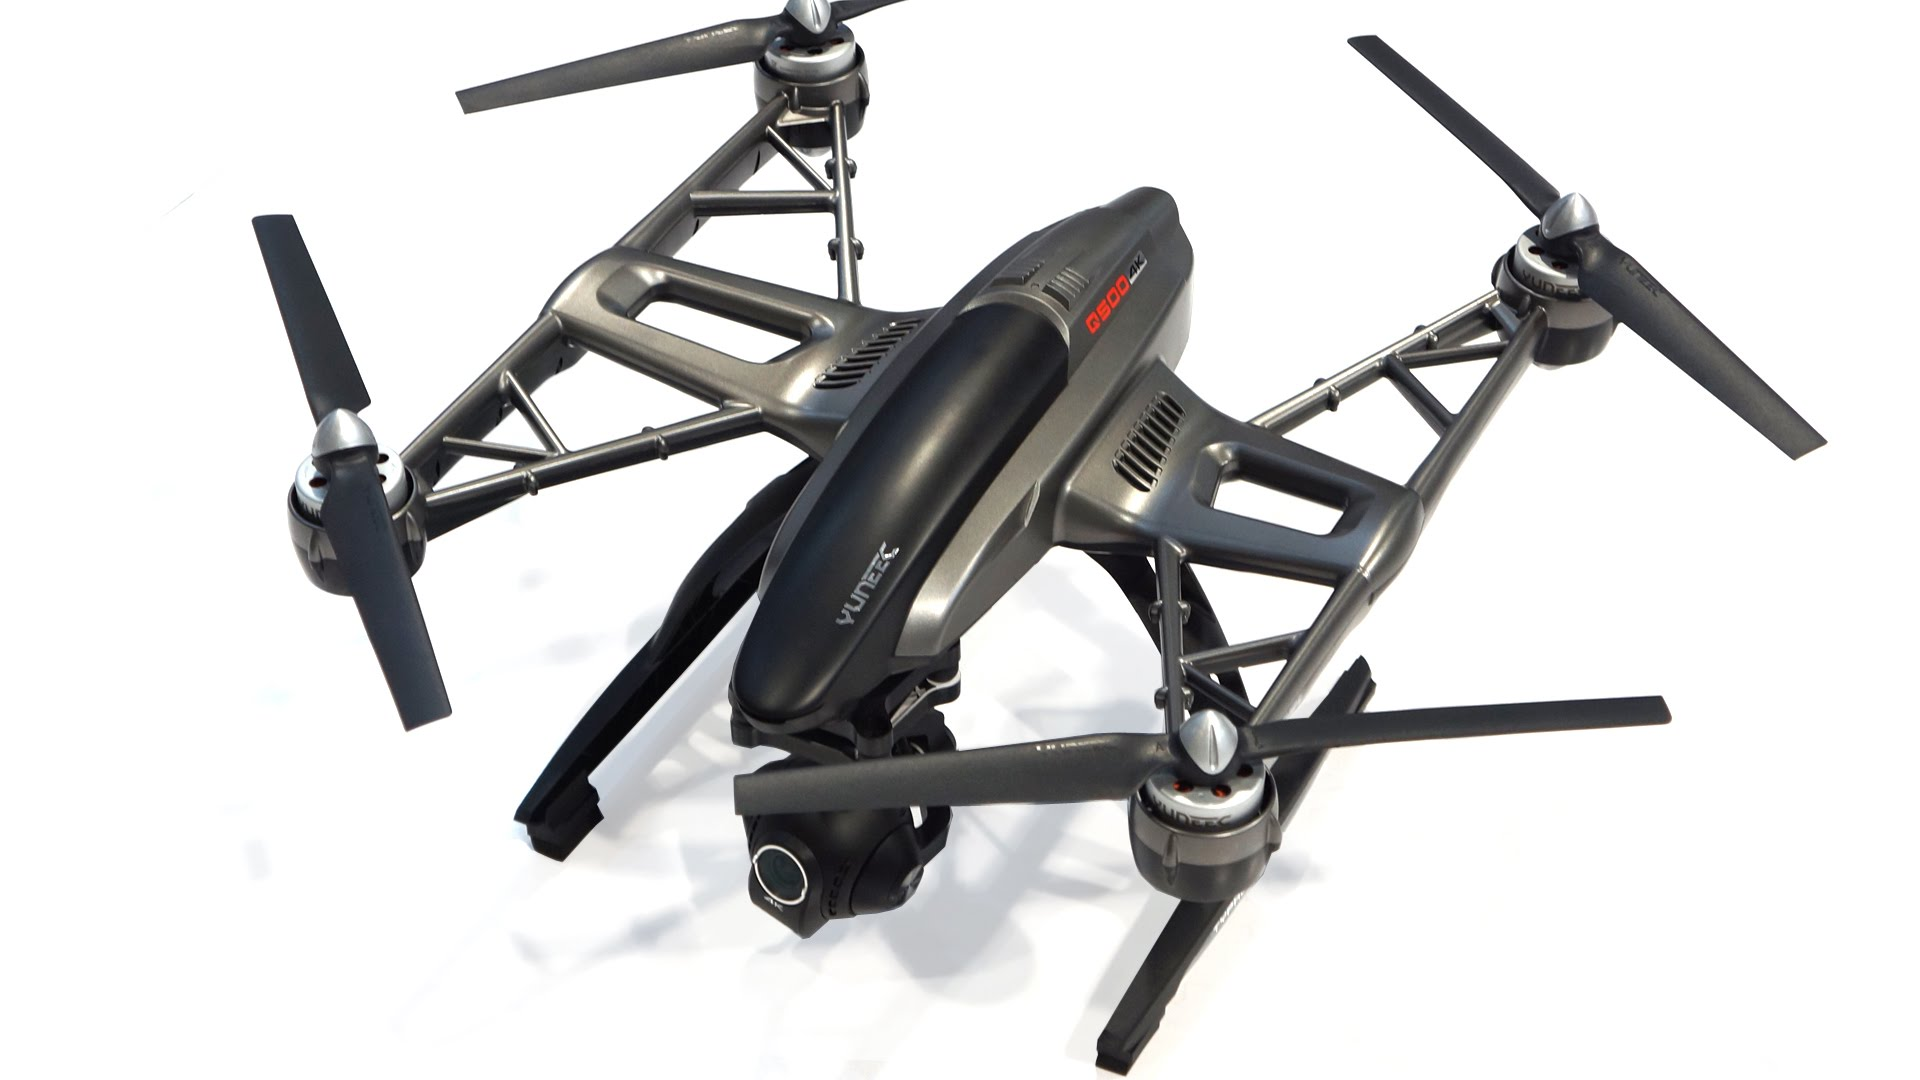
\includegraphics[width=8cm]{drone}
\label{fig:drone}
\caption{O drone utilizado para a gravação dos vídeos de teste.}
\centering
\end{figure}

Para a aquisição das imagens utilizadas para o treinamento da rede, o primeiro vídeo passou por um processo semelhante ao processo de calibração do programa final descrito no capítulo \ref{cap:solucao}. Duas áreas de interesse foram determinadas de forma idêntica ao processo de escolha de ROIs do programa. Em seguida cada ROI foi dividida em trinta seções verticais. Três quadros do vídeo foram escolhidos de forma aleatória. As imagens correspondentes a cada seção de cada quadro escolhido foram extraídas em arquivos separados. Dessa maneira, as imagens utilizadas para o treinamento da rede neural foram construídas da mesma maneira que as imagens que seriam alimentadas a ela para classificação no futuro.

\section{Treinamento da rede neural artificial}

Uma vez adquiridas as imagens a serem utilizadas para o treinamento, cada uma delas foi separada manualmente em uma das duas categorias:veículo ou vaga vazia. Ao todo foram utilizadas $57$ imagens classificadas como veículo(categoria 1) e $59$ imagens classificadas como vaga vazia(categoria 2) totalizando $116$ imagens. Foram extraídas as características de cada imagem da forma descrita na seção \ref{sec:extracao}. Os vetores $x_s$ obtidos foram então concatenados de forma a criar duas matrizes. A primeira de dimensões $6x57$ representava as \textit{features} das imagens de carros e a segunda de dimensões $6x59$ as características das imagens de vagas desocupadas.

\begin{figure}
\centering
\begin{subfigure}{.1\textwidth}
  \centering
  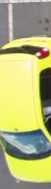
\includegraphics[width=.8\linewidth, height=5cm]{ocupada}
  \caption{}
  \label{fig:exemploRede:sub:ocupada}
\end{subfigure}%
\begin{subfigure}{.1\textwidth}
  \centering
  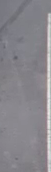
\includegraphics[width=.8\linewidth, height=5cm]{desocupada}
  \caption{}
  \label{fig:exemploRede:sub:desocupada}
\end{subfigure}
\centering
\caption{(a)Um exemplo de imagem classificada manualmente na classe 1.(b) Um exemplo de imagem classificada manualmente na classe 2.}
\label{fig:exemploRede}
\end{figure}

Para que pudesse ser feito o treinamento supervisionado da rede neural, duas matrizes de alvos foram construídas. Uma com dimensões $2x57$ e a outra com dimensões $2x59$. A primeira matriz com todas as colunas iguais a $\begin{psmallmatrix}1\\0\end{psmallmatrix}$ e a segunda com as colunas da forma $\begin{psmallmatrix}0\\1\end{psmallmatrix}$. Essas matrizes vão compor o gabarito utilizado para o treinamento supervisionado da rede.

As matrizes  de características de cada classe foram então concatenadas formando uma matriz de entrada $In_{6x116}$. O mesmo foi feito com as matrizes do gabarito, resultando na matriz $Target_{2x116}$. Em seguida as colunas dessas duas matrizes foram reorganizadas aleatoriamente, de forma que as mudanças feitas em $In$ fossem refletidas em $Out$, garantindo que não fosse perdida a relação entre as colunas de mesmo índice das matrizes. O resultado final deste processo é que cada coluna de $Target_{2x116}$ indica a classe da coluna correspondente de $In_{6x116}$.

Uma vez criadas essas duas matrizes, as entradas e seus respectivos alvos são separados em três conjuntos: o conjunto de treinamento, de validação e de testes. A divisão é feita de forma que $70\%$ das entradas são designadas ao conjunto de treinamento, $15\%$ designadas ao conjunto de validação e os $15\%$ restantes ao conjunto de testes. O conjunto de treinamento então é composto por duas matriz $Ti_{6x81}$ e $To_{2x81}$ que são iguais as primeira $81$ colunas de $In_{6x116}$ e $Target_{2x116}$ e representam os vetores descritores das entradas e seus gabaritos respectivamente. Os outros dois conjuntos são construídos de forma similar utilizando. O conjunto de validação é composto por matrizes de $18$ colunas e o de teste por matrizes de $17$ colunas.


A rede neural utilizada foi uma rede \textit{feed-forward} com três camadas. A camada oculta possui $15$ neurônios com função de ativação logística (\ref{eq:logistica}) e a camada de saída $2$ neurônios com função de ativação \textit{softmax} (\ref{eq:softmax}). A rede é submetida a um treinamento supervisionado com um limite de $1000$ iterações. Quando a situação de convergência é atingida, o treinamento para e o resultado é a rede final utilizada.


\section{Resultados Obtidos}

Para determinar a capacidade da programa de determinar se as seções verticais estão ocupadas ou livres, os resultados obtidos pelo programa foram comparados com os resultados que eram esperados de observadores humanos. Foram apresentados a três observadores, que chamaremos pelas iniciais F, M e P, um conjunto de oito vídeos que mostravam veículos estacionando ou saindo de vagas em um estacionamento descoberto. As áreas de interesse do vídeo foram definidas previamente e divididas em $30$ seções verticais. Dessa forma, todos os observadores e o programa analisaram seções verticais idênticas. 

Cada um dos observadores receberam as seguintes instruções:

\begin{itemize}
  \item As regiões de interesse e as seções são numeradas como indicado na figura \ref{instrucoes};
	\item Uma seção ocupada é aquela cuja maior parte de sua área está ocupada por um veículo;
	\item No momento inicial do vídeo ($0$ segundos), indique quais seções verticais estão ocupadas através do número das ROI e das seções, as outras serão assumidas como livres;
	\item Se a qualquer momento o estado de ocupação de uma seção mudar, indique o tempo da mudança, a seção onde ocorreu a mudança e a natureza da mudança(ocupada ou liberada).
\end{itemize}

\begin{figure}
\centering
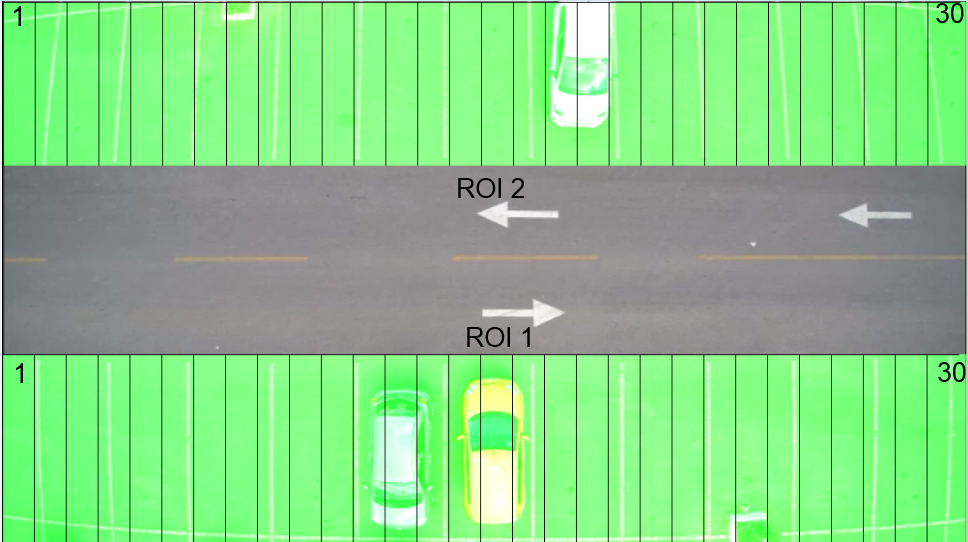
\includegraphics[width=8cm]{instrucoes}
\centering
\caption{Figura mostrando a divisão das ROIs e numeração das seções nos vídeos mostrados para os observadores humanos}
\label{fig:instrucao}
\end{figure}

Cada observador assistiu aos vídeos sozinho, sem interferência externa e sem conhecimento dos resultados do programa. De fato, a fim de evitar interferência, o programa só foi executado sobre os casos de teste após todos os observadores escolhidos terem entregado os resultados que obteram.

Para os testes apresentados a seguir, serão observadas somente aquelas seções que o programa ou os observadores determinaram como ocupadas. As demais seções serão consideradas livres. Chamaremos de um \textit{acerto} sempre que em um determinado segundo $t$, o programa e um observador concordam quanto a ocupação de uma seção vertical. Sendo assim, o programa pode atingir um máximo de $60$ acertos por segundo. A indicação da ocupação das seções pelos observadores não foi definida a cada segundo, mas considera-se que entre duas acusações de mudança de estado a ocupação das seções permanece a mesma. Sendo assim, podemos utilizar esses momentos para definir a ocupação em cada segundo do vídeo. Por exemplo, se um observador disser que a seção $10$ estava ocupada no momento inicial do vídeo e depois indicar que a mesma sessão foi liberada aos $8s$, a seção será considerada ocupada durante todos os momentos deste intervalo. 

Em seguida serão apresentados como um dos vídeos utilizados para os testes. Cada caso iniciará com uma breve descrição do movimento dos veículos no vídeo, a duração do vídeo e o número de acertos possíveis, seguidos de quatro tabelas, uma para cada observador e uma quarta para o programa. As tabelas indicam o tempo onde foram acusadas mudanças de estado nas seções. A primeira linha da tabela indica as seções ocupadas no momento inicial do vídeo e cada linha subsequente indica um momento em segundos quando houve mudança de estado de pelo menos uma seção e a ROI e número das seções. Finalmente, será calculada uma taxa de acerto que compara o desempenho do programa a cada observador e uma taxa final de acerto média para o caso de teste. A taxa de acerto para cada observador é calculada pela razão entre o número de acertos do programa e o número de acertos possíveis para o caso de teste e a taxa de acerto média é a média aritmética entre estes valores. Ao final destas seções uma breve análise dos resultados dos casos de teste será apresentada. Para que o leitor possa compara o desempenho do programa com suas próprias impressões, uma imagem dos momentos iniciais e finais de cada vídeo será mostrada junto de cada análise.


 
\subsection{Vídeo 1}

No primeiro caso de testes, o vídeo começa com um estacionamento vazio. Depois de alguns segundos um único veículo de cor branca entra na cena pela direita e estaciona em uma vaga na parte inferior da imagem. O vídeo tem $15s$ de duração, totalizando $900$ acertos possíveis.

\begin{figure}[!h]
\centering
\begin{subfigure}{.5\textwidth}
\centering
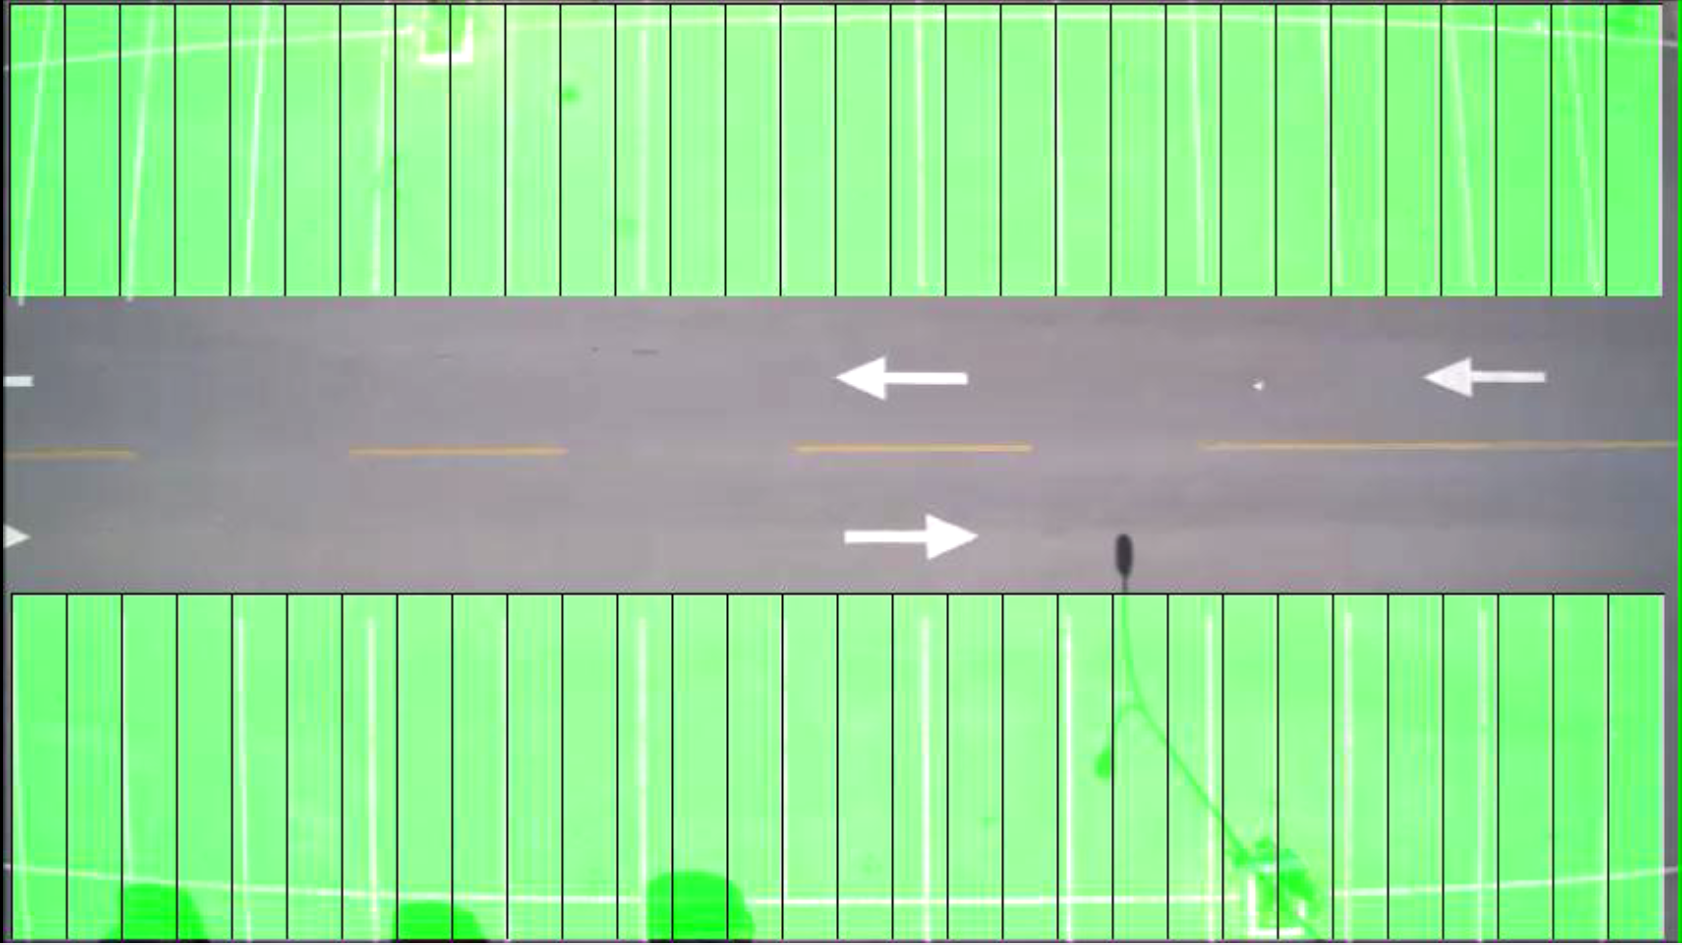
\includegraphics[width=.8\linewidth]{Video1Inicio}
\caption{}
\end{subfigure}\
\begin{subfigure}{.5\textwidth}
\centering
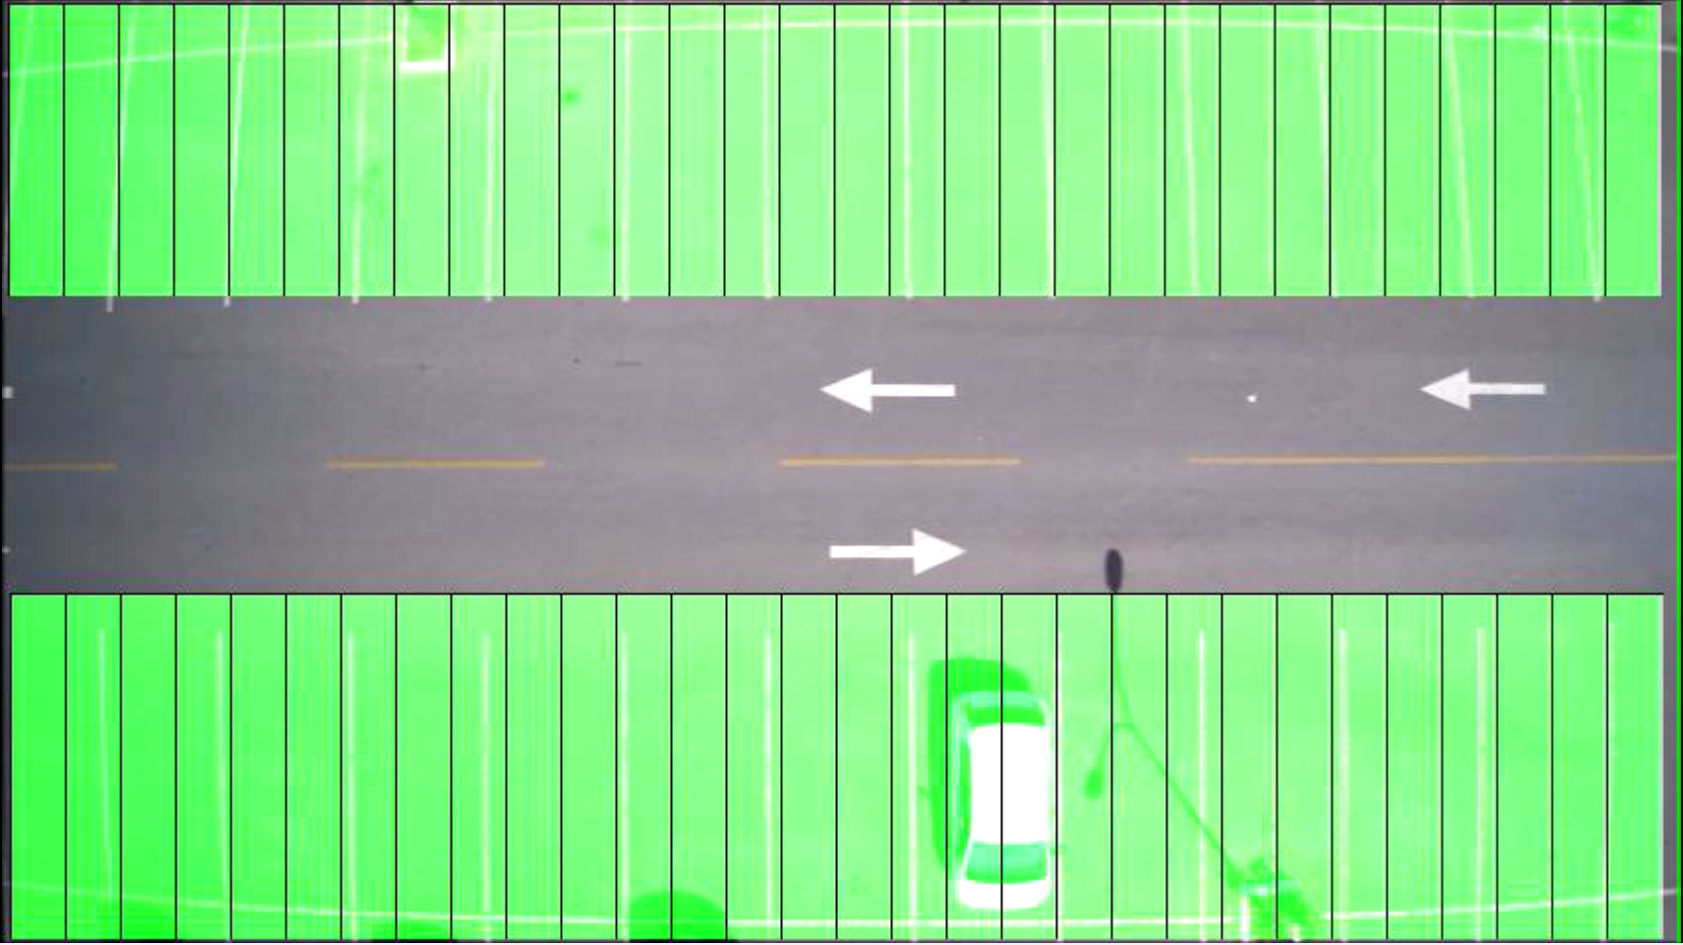
\includegraphics[width=.8\linewidth]{Video1Fim}
\caption{}
\end{subfigure}
\centering
\caption{(a) O momento inicial do vídeo 1. (b) O momento final do vídeo 1}%
\label{}%
\end{figure}


\begin{center}
\begin{tabular}{|c||c|}
\hline
\multicolumn{2}{|c|}{Observador F}  \\ \hline \hline
Tempo(s) & Acontecimento \\ \hline
0 & Nenhuma seção ocupada \\ \hline
10 & ROI 2: Seções 18 e 19 ocupadas. \\
\hline
\end{tabular}
\end{center}

\begin{center}
\begin{tabular}{|c||c|}
\hline
\multicolumn{2}{|c|}{Observador P}  \\ \hline \hline
Tempo(s) & Acontecimento \\ \hline
0 & Nenhuma seção ocupada \\ \hline
10 & ROI 2: Seções 18 e 19 ocupadas. \\
\hline
\end{tabular}
\end{center}

\begin{center}
\begin{tabular}{|c||c|}
\hline
\multicolumn{2}{|c|}{Observador M}  \\ \hline \hline
Tempo(s) & Acontecimento \\ \hline
0 & Nenhuma seção ocupada \\ \hline
9 & ROI 2: Seções 18 e 19 ocupadas. \\
\hline
\end{tabular}
\end{center}

\begin{center}
\begin{tabular}{|c||c|}
\hline
\multicolumn{2}{|c|}{Programa}  \\ \hline \hline
Tempo(s) & Acontecimento \\ \hline
0 & ROI 2:Seção 3 ocupada. \\ \hline
10 & ROI 2: Seções 18 e 19 ocupadas. \\ \hline
14 & ROI 2: Seção 3 liberada. \\
\hline
\end{tabular}
\end{center}

\begin{center}
\begin{tabular}{|c||c||c|}
\hline
Observador & Acertos & Taxa de acertos \\ \hline
F & 886 & 98,44\% \\  \hline
P & 886 & 98,44\% \\ \hline
M & 884 & 98,22\% \\ \hline
Média & 885,3 & 98,37\% \\
\hline
\end{tabular}
\end{center}

Neste caso de testes, o programa classifica errôneamente a seção $3$ da ROI $2$ durante quase toda a duração do vídeo. Apesar de persistente este erro tem pouca influência na indicação do número de vagas ocupadas, pois uma seção ocupada solitária não é suficiente para que o programa diminua o número de vagas livres.

Em relação ao observador M, o programa apresentou um atraso de $1s$ na classificação das seções $18$ e $19$ da ROI $2$, um atraso considerado aceitável, principalmente se considerarmos que o programa classificou estas mesmas seções no mesmo momento que os outros dois observadores.

\subsection{Vídeo 2}

Neste vídeo, um carro branco está estacionado no conjunto inferior de vagas. Um veículo cinza entra pela direita e estaciona no conjunto superior de vagas. O vídeo tem uma duração de $10s$, totalizando $600$ acertos possíveis.

\begin{figure}[!h]
\centering
\begin{subfigure}{.5\textwidth}
\centering
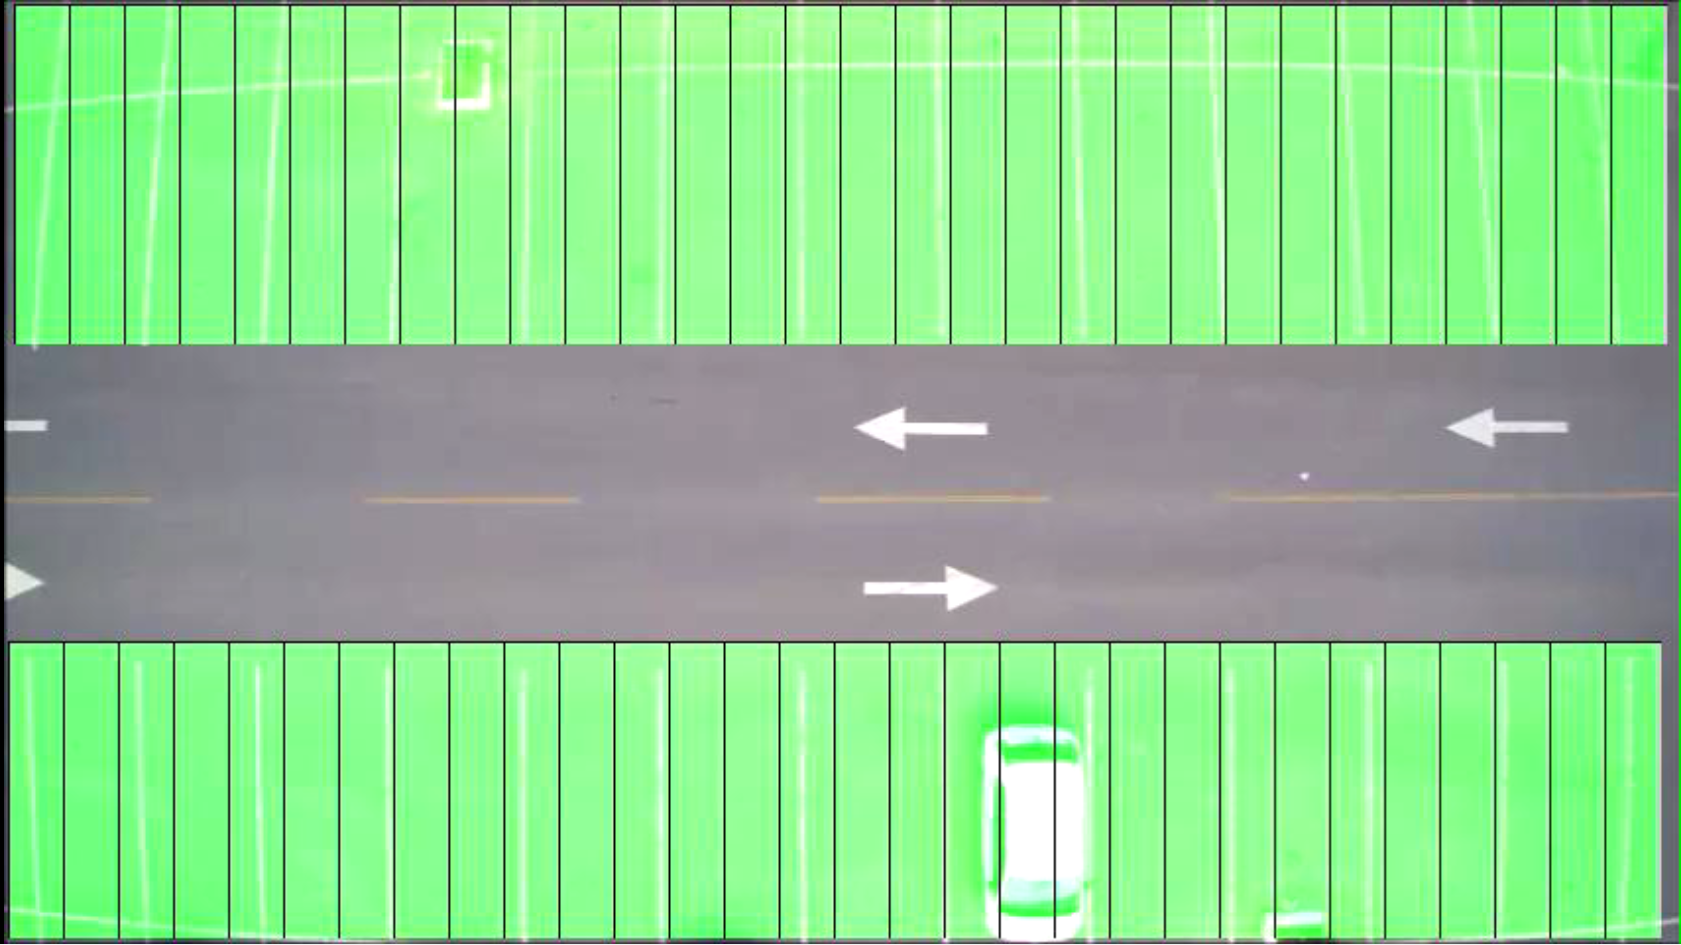
\includegraphics[width=.8\linewidth]{Video2Inicio}
\caption{}
\end{subfigure}\
\begin{subfigure}{.5\textwidth}
\centering
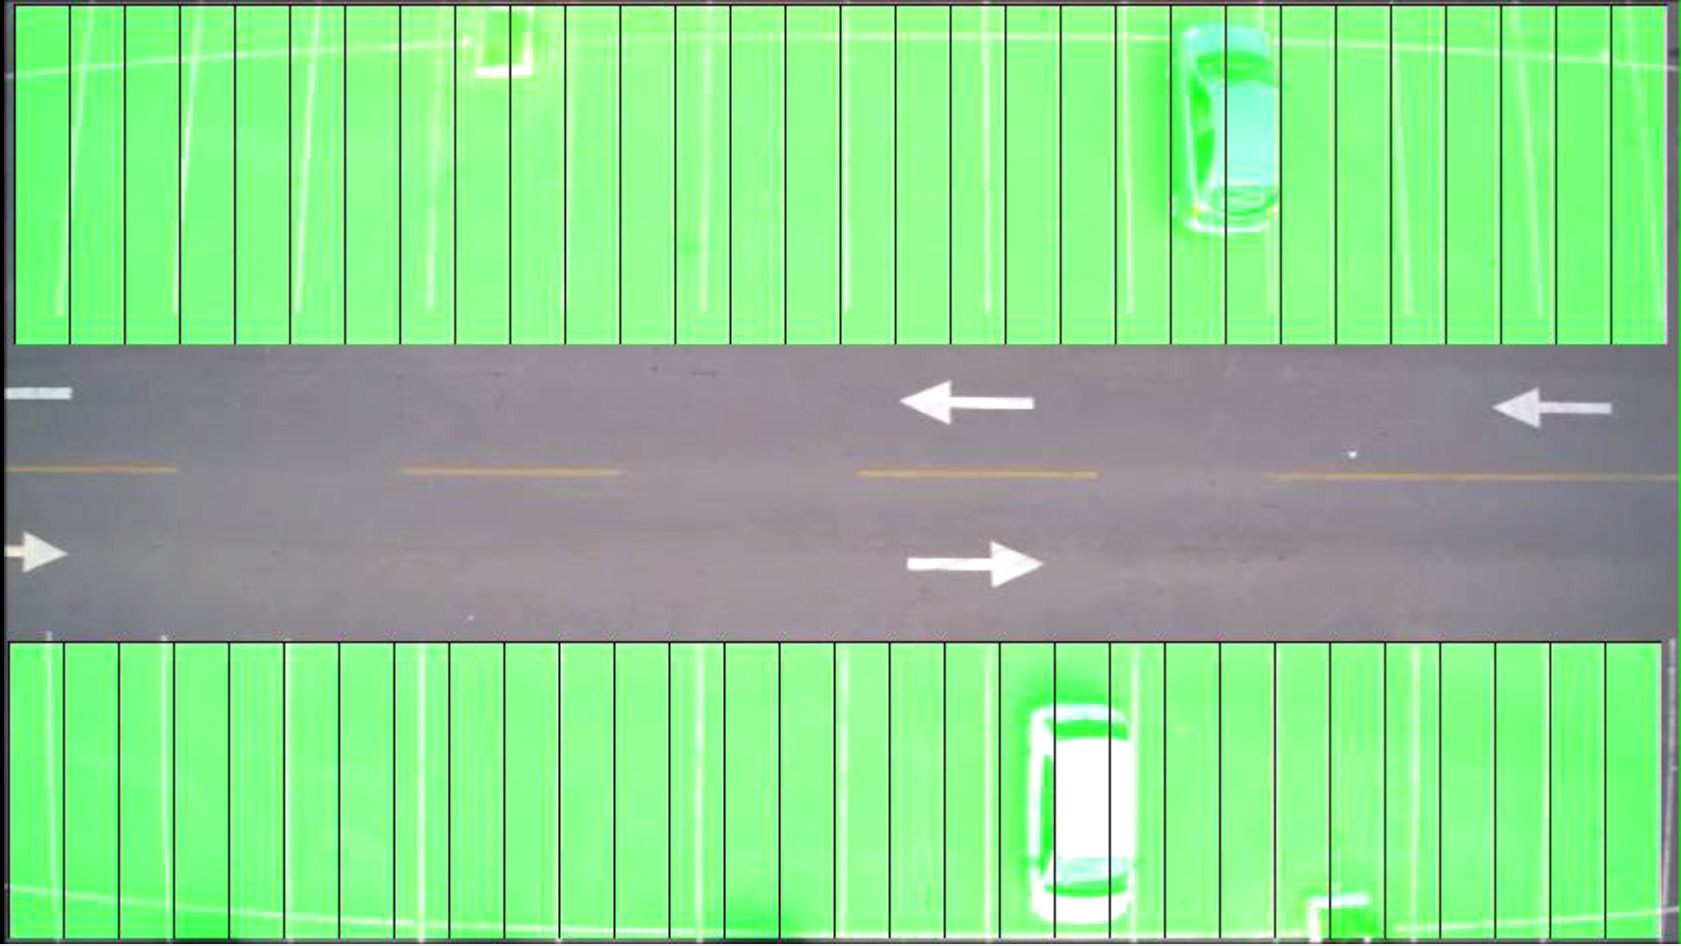
\includegraphics[width=.8\linewidth]{Video2Fim}
\caption{}
\end{subfigure}
\centering
\caption{(a) O momento inicial do vídeo 2. (b) O momento final do vídeo 2}%
\label{}%
\end{figure}


\begin{center}
\begin{tabular}{|c||c|}
\hline
\multicolumn{2}{|c|}{Observador F}  \\ \hline \hline
Tempo(s) & Acontecimento \\ \hline
0 & ROI 2: Seções 19 e 20 ocupadas \\ \hline
6 & ROI 1: Seções 21,22 e 23 ocupadas. \\
\hline
\end{tabular}
\end{center}

\begin{center}
\begin{tabular}{|c||c|}
\hline
\multicolumn{2}{|c|}{Observador P}  \\ \hline \hline
Tempo(s) & Acontecimento \\ \hline
0 & ROI 2: Seções 19 e 20 ocupadas \\ \hline
6 & ROI 1: Seções 20,21,22 ocupadas. \\
\hline
\end{tabular}
\end{center}

\begin{center}
\begin{tabular}{|c||c|}
\hline
\multicolumn{2}{|c|}{Observador M}  \\ \hline \hline
Tempo(s) & Acontecimento \\ \hline
0 & ROI 2: Seções 19 e 20 ocupadas \\ \hline
6 & ROI 1: Seções 21,22 e 23 ocupadas. \\
\hline
\end{tabular}
\end{center}

\begin{center}
\begin{tabular}{|c||c|}
\hline
\multicolumn{2}{|c|}{Programa}  \\ \hline \hline
Tempo(s) & Acontecimento \\ \hline
0 & ROI 2: Seções 18,19 e 20 ocupadas. \\ \hline
6 & ROI 1: Seções 21 e 22 ocupadas. \\ \hline
\hline
\end{tabular}
\end{center}

\begin{center}
\begin{tabular}{|c||c||c|}
\hline
Observador & Acertos & Taxa de acertos \\ \hline
F & 586 & 97,66\% \\  \hline
P & 586 & 97,66\% \\ \hline
M & 586 & 97,66\% \\ \hline
Média & 586 & 97,66\% \\
\hline
\end{tabular}
\end{center}

Neste caso de testes, houve discordância entre os observadores sobre as seções ocupadas pelo carro cinza na parte superior do vídeo. Porém o programa classificou como ocupadas as seções onde houve consenso entre os observadores.

O programa também classificou errôneamente a seção $18$ do ROI $2$ no momento inicial do vídeo. Novamente ele acerta nas seções onde há consenso entre os observadores. O erro é mais aceitável que o erro que ocorreu no vídeo $1$, por causa da proximidade da seção mal-classificada das seções onde houve acerto.

\subsection{Vídeo 3}

Neste vídeo, dois carros se encontram no estacionamento. Um veículo amarelo entra pela direita e estaciona na seção superior das vagas. O veículo branco sai pela parte de baixo da tela. Ele tem duração de $20s$ totalizando $1200$ acertos possíveis.

\begin{figure}[!h]
\centering
\begin{subfigure}{.5\textwidth}
\centering
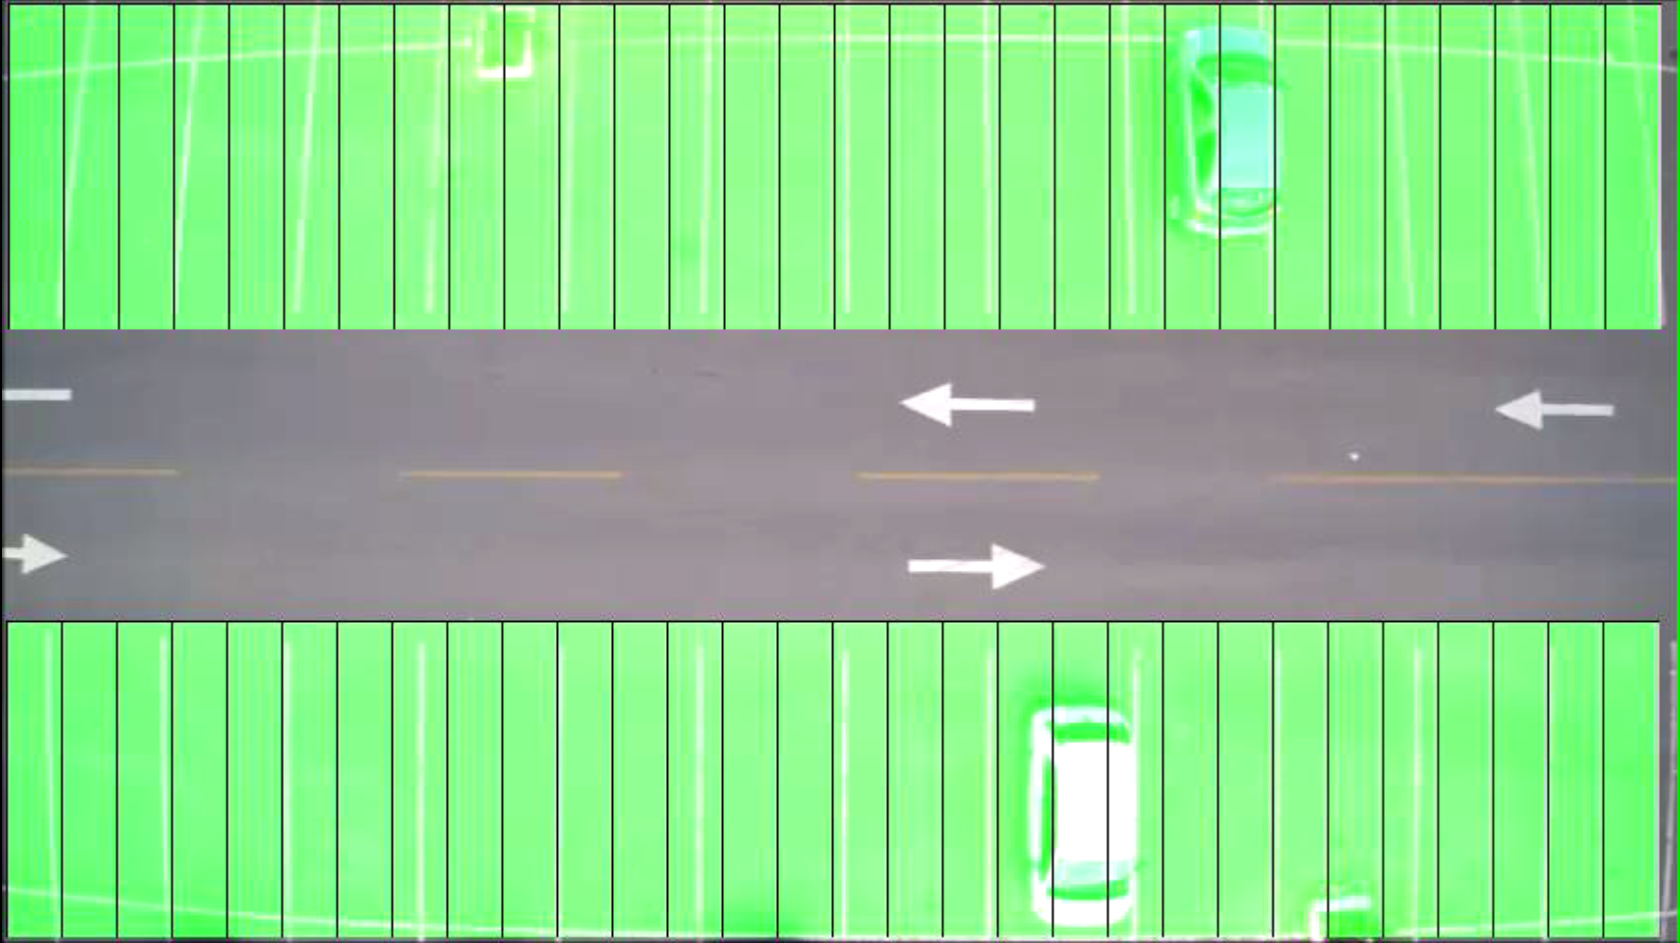
\includegraphics[width=.8\linewidth]{Video3Inicio}
\caption{}
\end{subfigure}\
\begin{subfigure}{.5\textwidth}
\centering
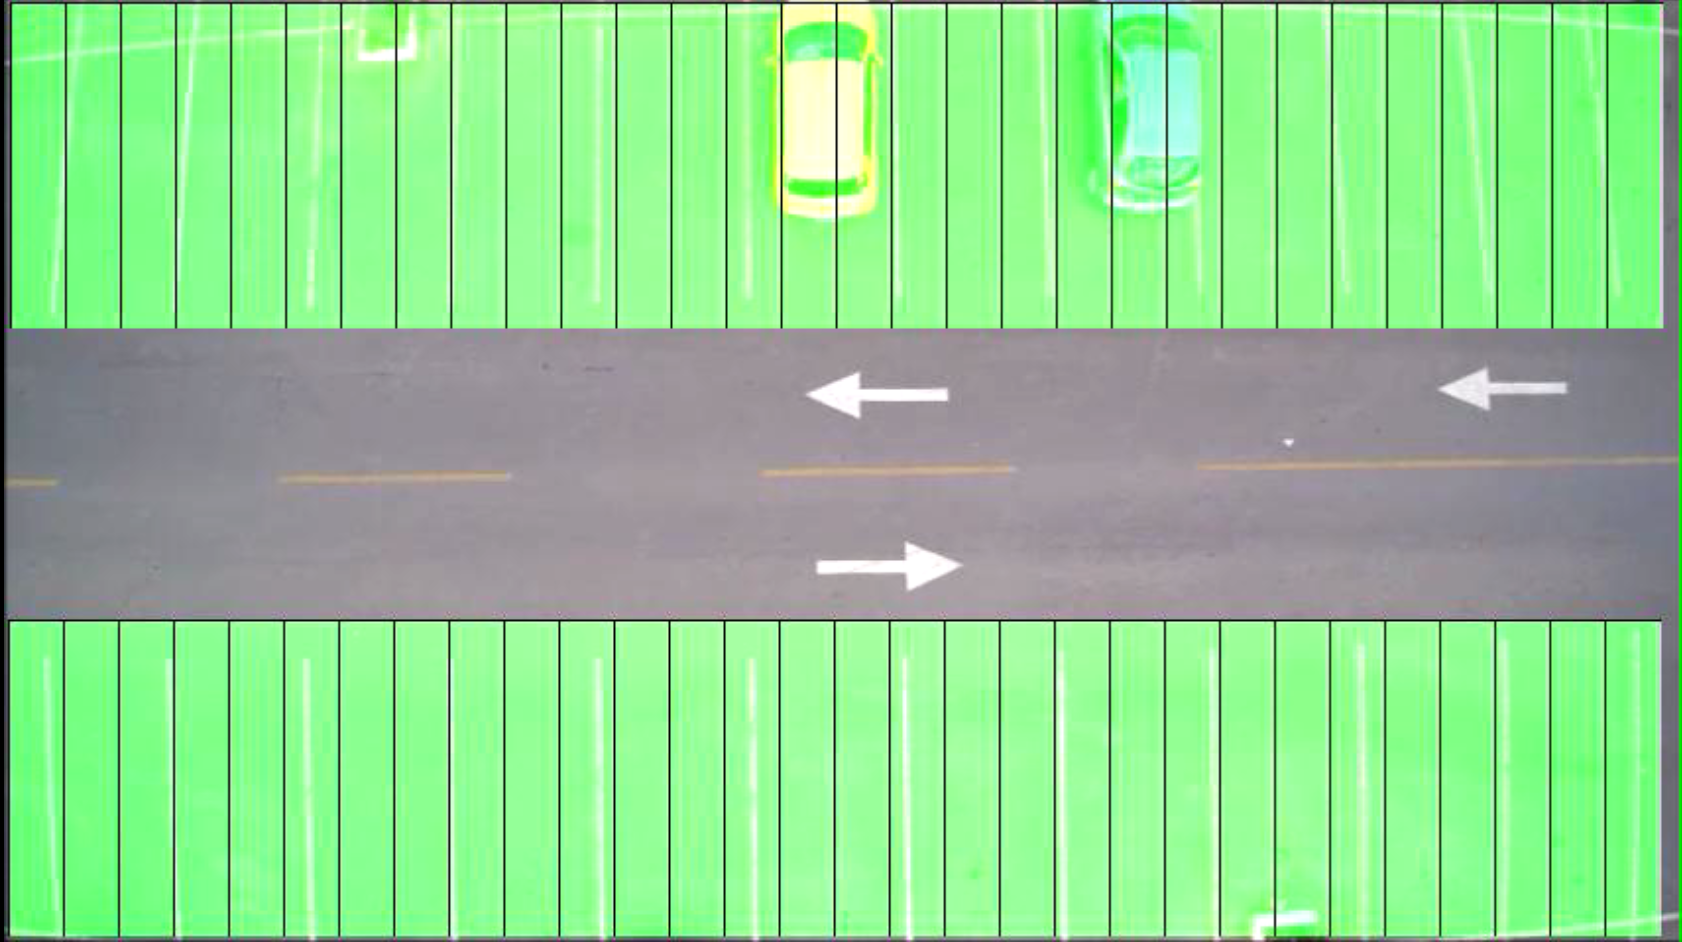
\includegraphics[width=.8\linewidth]{Video3Fim}
\caption{}
\end{subfigure}
\centering
\caption{(a) O momento inicial do vídeo 3. (b) O momento final do vídeo 3}%
\label{}%
\end{figure}

\begin{center}
\begin{tabular}{|c||c|}
\hline
\multicolumn{2}{|c|}{Observador F}  \\ \hline \hline
Tempo(s) & Acontecimento \\ \hline
0 & ROI 1: Seções 22 e 23 ocupadas. \\
 & ROI 2: 19,20 e 21 ocupadas \\ \hline
8 & ROI 1: Seções 16 e 17 ocupadas. \\ \hline
13 & ROI 2: Seções 18 e 19 liberadas. \\
\hline
\end{tabular}
\end{center}

\begin{center}
\begin{tabular}{|c||c|}
\hline
\multicolumn{2}{|c|}{Observador P}  \\ \hline \hline
Tempo(s) & Acontecimento \\ \hline
0 & ROI 1: Seções 22 e 23 ocupadas. \\
 & ROI 2: 20 e 21 ocupadas \\ \hline
9 & ROI 1: Seções 15,16 e 17 ocupadas. \\
\hline
\end{tabular}
\end{center}

\begin{center}
\begin{tabular}{|c||c|}
\hline
\multicolumn{2}{|c|}{Observador M}  \\ \hline \hline
Tempo(s) & Acontecimento \\ \hline
0 & ROI 1: Seções 22 e 23 ocupadas. \\
 & ROI 2: 20 e 21 ocupadas \\ \hline
8 & ROI 1: Seções 15,16 e 17 ocupadas. \\ \hline
14 & ROI 2: Seções 17,18 e 19 liberadas \\
\hline
\end{tabular}
\end{center}

\begin{center}
\begin{tabular}{|c||c|}
\hline
\multicolumn{2}{|c|}{Programa}  \\ \hline \hline
Tempo(s) & Acontecimento \\ \hline
0 & ROI 1: Seções 22 e 23 ocupadas. \\
 & ROI 2: 19,20 e 21 ocupadas \\ \hline
1 & ROI 1: Seção 23 liberada. \\ \hline
2 & ROI 1: Seção 23 ocupada. \\ \hline
4 & ROI 1: Seção 23 liberada. \\ \hline
8 & ROI 1: Seções 16 e 17 ocupadas. \\ \hline
9 & ROI 2: Seção 21 liberada. \\ 
 & ROI 2: Seções 18 e 24 ocupadas \\ \hline
11 & ROI 1: Seção 20 ocupada. \\ 
 & ROI 2: Seção 24 liberada. \\ \hline
13 & ROI 1: Seção 20 liberada. \\
 & ROI 2: Seção 18,19 e 20 liberada. \\ \hline
16 & ROI 1: Seção 20 ocupada. \\ \hline
19 & ROI 1: Seção 20 liberada. \\
\hline
\end{tabular}
\end{center}

\begin{center}
\begin{tabular}{|c||c||c|}
\hline
Observador & Acertos & Taxa de acertos \\ \hline
F & 1165 & 97,08\% \\  \hline
P & 1113 & 92,75\% \\ \hline
M & 1136 & 94,66\% \\ \hline
Média & 1138 & 94,83\% \\
\hline
\end{tabular}
\end{center}

Esse caso de teste possui alguns problemas causados principalmente por causa da movimentação do \textit{drone} no momento da gravação. Essa movimentação faz com que partes da imagem passem a ocupar seções diferentes, criando algumas incosistências. Repare que por volta dos $14s$ dois dos observadores disseram que a seção $18$ da ROI $2$ foi liberada, apesar de nunca terem acusado que ela estava ocupada anteriormente. Essa inconsistência ocorre porque entre o início do vídeo esse momento, o \textit{drone} utilizado para a gravação se movimenta e faz com que o veículo que estava ocupando as  seções $19$ e $20$ ocupe as seções $18$ e $19$. Esse problema acontece em outros casos de teste em menor proporção.

Apesar destes problemas, o teste sobre esse vídeo ainda possui resultados interessantes e úteis. Uma vantagem do uso de um sistema automatizado se mostra neste caso de teste. O observador \textit{P} não percebeu que um veículo saia da tela por volta dos $14$ segundos e por isso não acusou a mudança de estado de nenhuma seção nesse momento. Uma falha que não ocorre no programa. 

Através deste caso também percebe-se que o programa tem dificuldade em classificar corretamente as seções ocupadas pelo veículo cinza na ROI $1$, evidenciada principalmente pela flutuação da classificação das seções $23$ e $20$.



\subsection{Vídeo 4}

Neste vídeo, o veículo branco entra em cena pela parte superior da tela e estaciona entre os outros dois carros. O carro cinza sai da vaga que ocupava e estaciona em uma na área inferior. Duração de $30s$, portanto $1800$ possíveis acertos.

\begin{figure}[!h]
\centering
\begin{subfigure}{.5\textwidth}
\centering
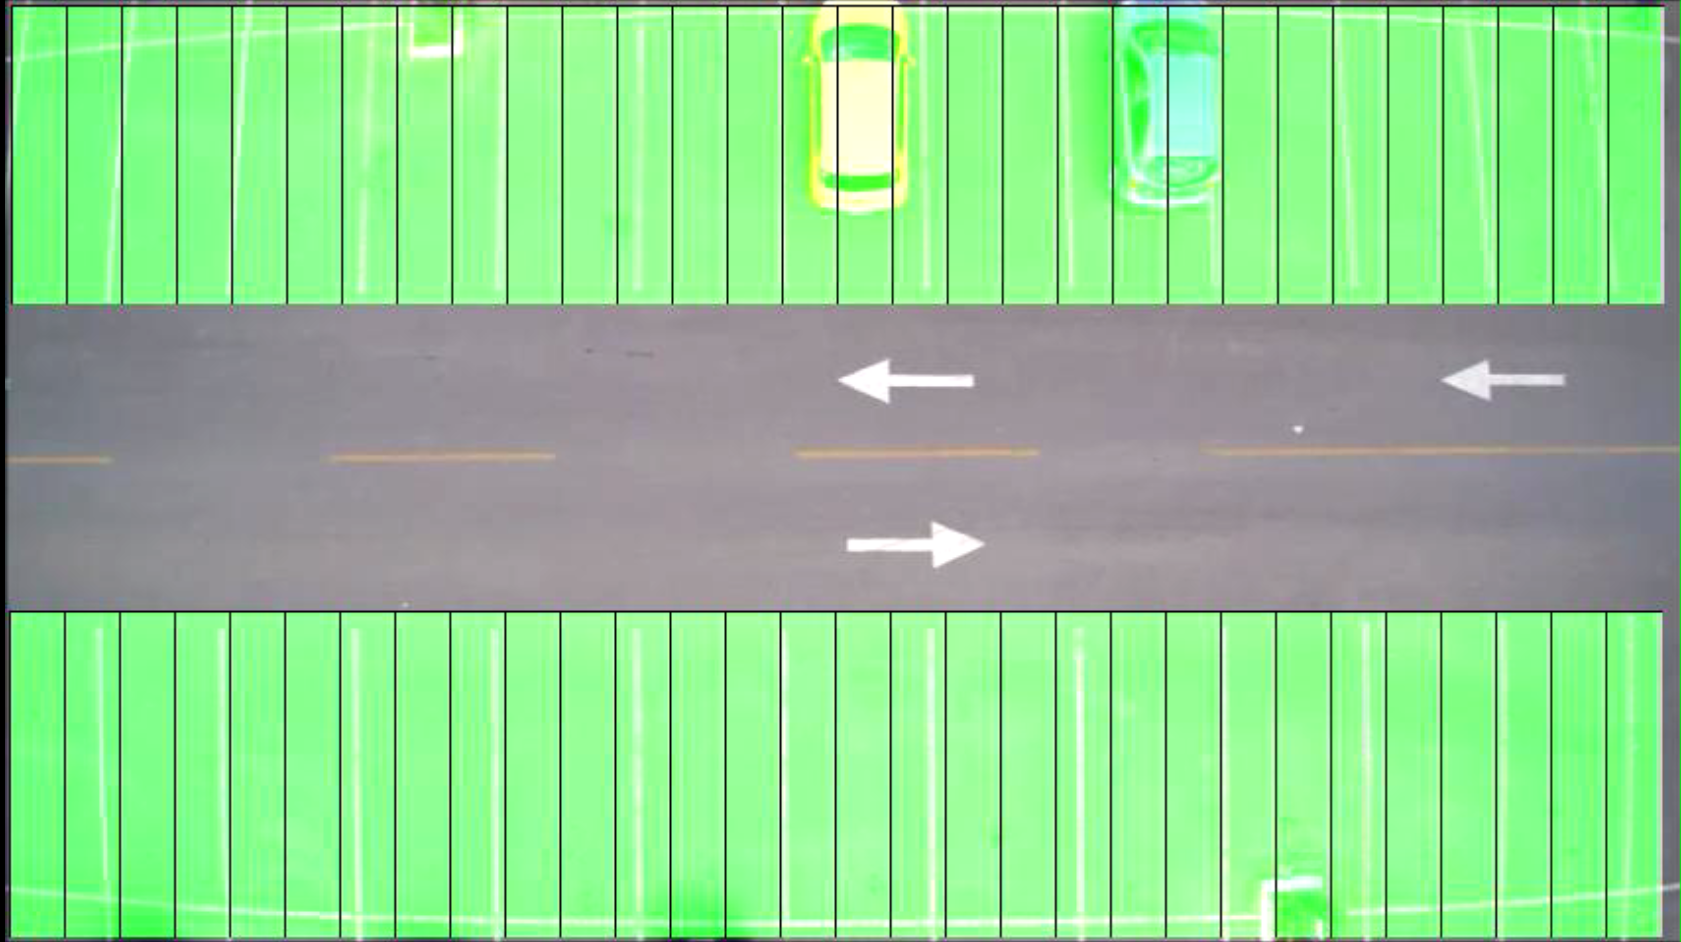
\includegraphics[width=.8\linewidth]{Video4Inicio}
\caption{}
\end{subfigure}\
\begin{subfigure}{.5\textwidth}
\centering
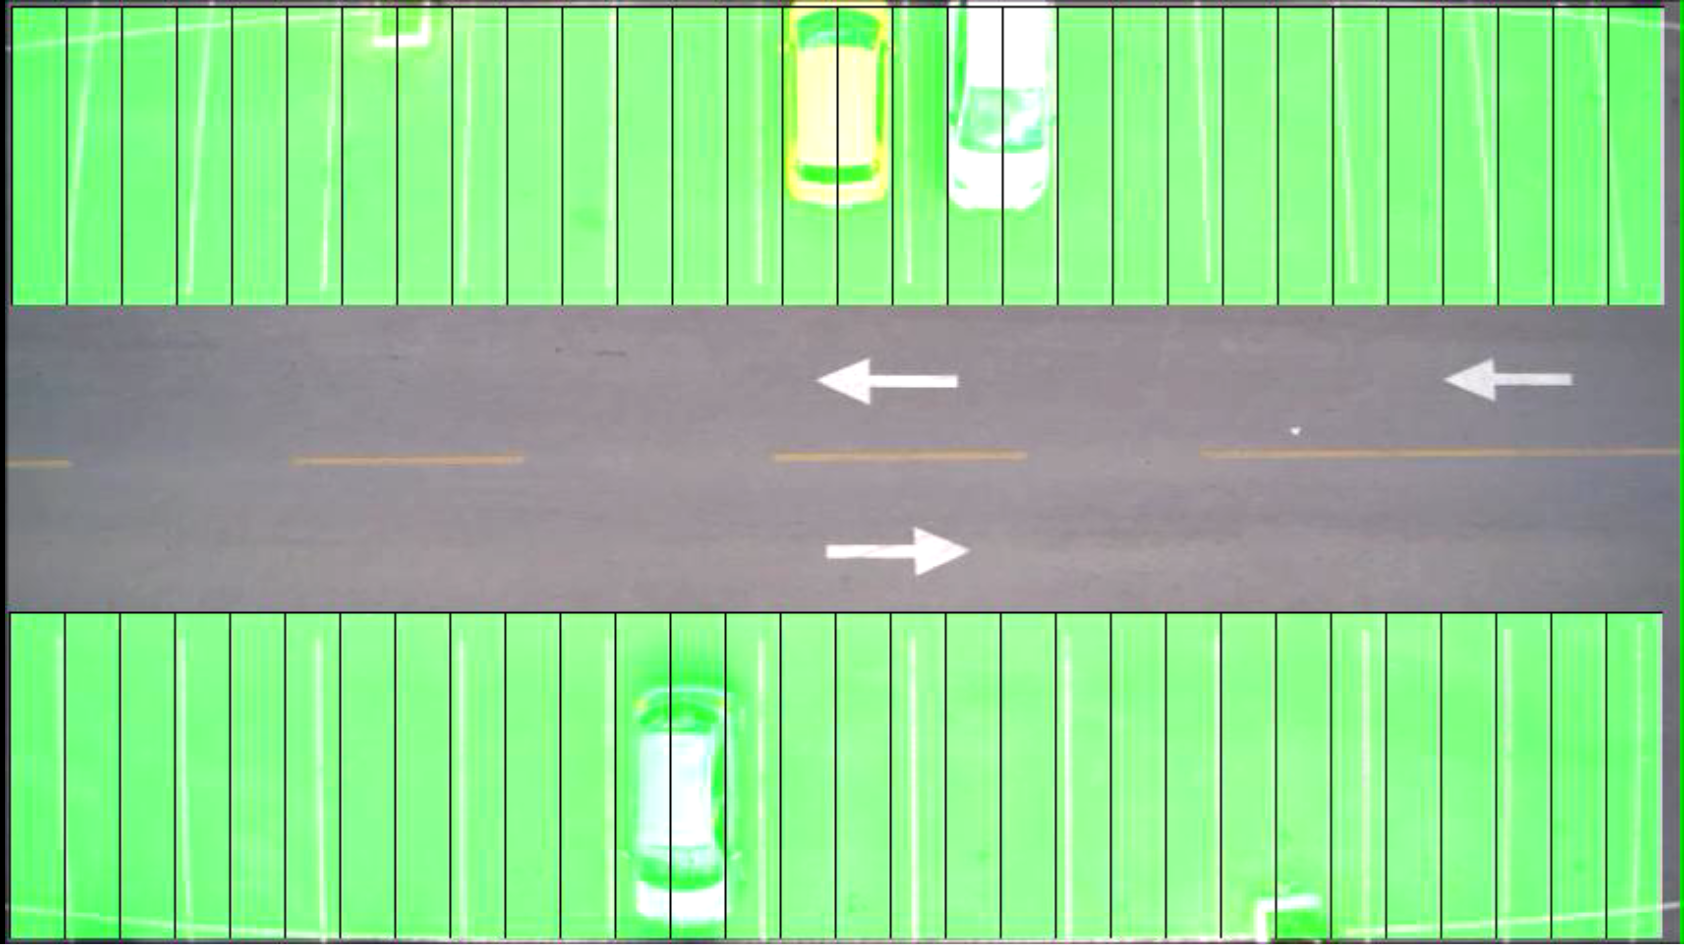
\includegraphics[width=.8\linewidth]{Video4Fim}
\caption{}
\end{subfigure}
\centering
\caption{(a) O momento inicial do vídeo 4. (b) O momento final do vídeo 4}%
\label{}%
\end{figure}

\begin{center}
\begin{tabular}{|c||c|}
\hline
\multicolumn{2}{|c|}{Observador F}  \\ \hline \hline
Tempo(s) & Acontecimento \\ \hline
0 & ROI 1: Seções 15,16,21 e 22 ocupadas. \\ \hline
7 & ROI 1: Seções 19 e 20 ocupadas. \\ \hline
16 & ROI 1: Seções 21 e 22 liberadas. \\ \hline
28 & ROI 2: Seções 12 e 13 ocupadas. \\
\hline
\end{tabular}
\end{center}

\begin{center}
\begin{tabular}{|c||c|}
\hline
\multicolumn{2}{|c|}{Observador P}  \\ \hline \hline
Tempo(s) & Acontecimento \\ \hline
0 & ROI 1: Seções 15,16,17,20 e 21 ocupadas. \\ \hline
8 & ROI 1: Seções 18 e 19 ocupadas. \\ \hline
18 & ROI 1: Seções 21 e 22 liberadas \\ \hline
29 & ROI 2: 12,13 e 14 ocupadas \\
\hline
\end{tabular}
\end{center}

\begin{center}
\begin{tabular}{|c||c|}
\hline
\multicolumn{2}{|c|}{Observador M}  \\ \hline \hline
Tempo(s) & Acontecimento \\ \hline
0 & ROI 1: Seções 15,16,20 e 21 ocupadas. \\ \hline
6 & ROI 1: Seções 18 e 19 ocupadas. \\ \hline
17 & ROI 1: Seções 21 e 22 liberadas \\ \hline
28 & ROI 2: Seções 12,13 e 14 ocupadas \\
\hline
\end{tabular}
\end{center}

\begin{center}
\begin{tabular}{|c||c|}
\hline
\multicolumn{2}{|c|}{Programa}  \\ \hline \hline
Tempo(s) & Acontecimento \\ \hline
0 & ROI 1: Seções 15,16,20 e 21 ocupadas. \\ \hline
6 & ROI 1: Seções 18 e 19 ocupadas. \\ \hline
11 & ROI 1: Seção 22 ocupada. \\ \hline
14 & ROI 1: Seção 22 liberada. \\ \hline
23 & ROI 1: Seção 20 liberada. \\ \hline
28 & ROI 2: Seções 12 e 13 ocupadas. \\
\hline
\end{tabular}
\end{center}

\begin{center}
\begin{tabular}{|c||c||c|}
\hline
Observador & Acertos & Taxa de acertos \\ \hline
F & 1750 & 97,22\% \\  \hline
P & 1749 & 97,16\% \\ \hline
M & 1772 & 98,44\% \\ \hline
Média & 1757 & 97,61\% \\
\hline
\end{tabular}
\end{center}

Este vídeo reforça a dificuldade do programa de classificar corretamente as seções ocupadas pelo veículo cinza. Porém a dificuldade parece não acontecer quando este carro estaciona na região inferior, quando o programa consegue que o veículo ocupa as mesmas seções que os observadores humanos.


\subsection{Vídeo 5}

Um veículo desocupa a sua vaga sainda pela parte superior da tela. Duração de $10s$ ou $600$ possíveis acertos.

\begin{figure}[!h]
\centering
\begin{subfigure}{.5\textwidth}
\centering
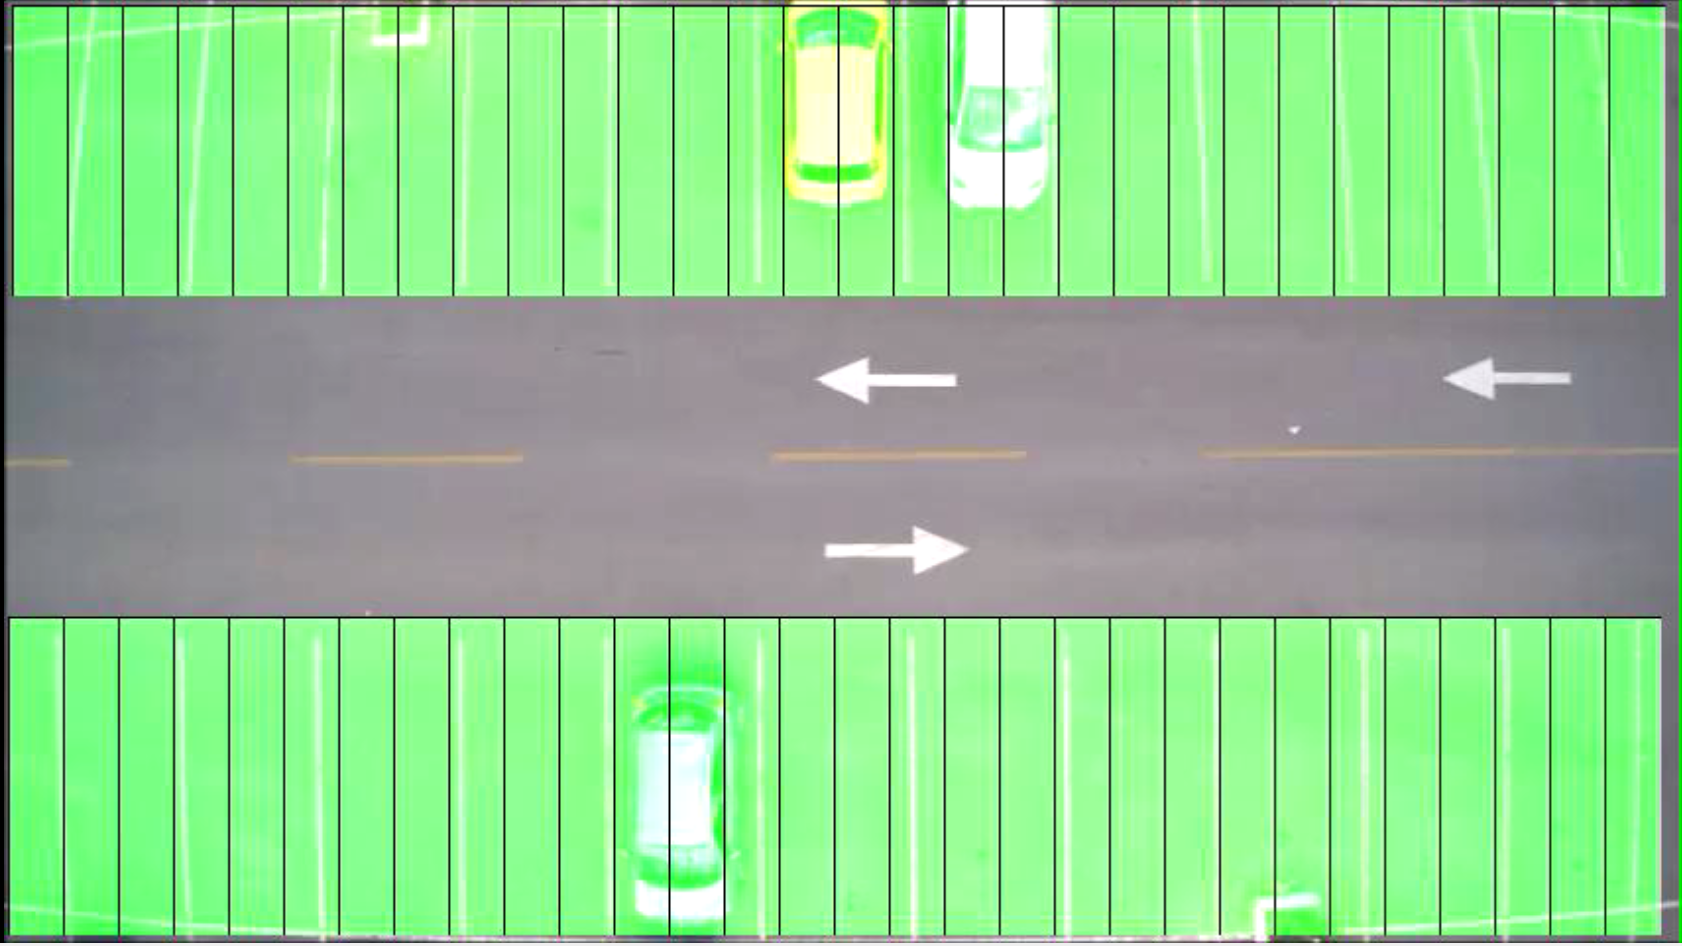
\includegraphics[width=.8\linewidth]{Video5Inicio}
\caption{}
\end{subfigure}\
\begin{subfigure}{.5\textwidth}
\centering
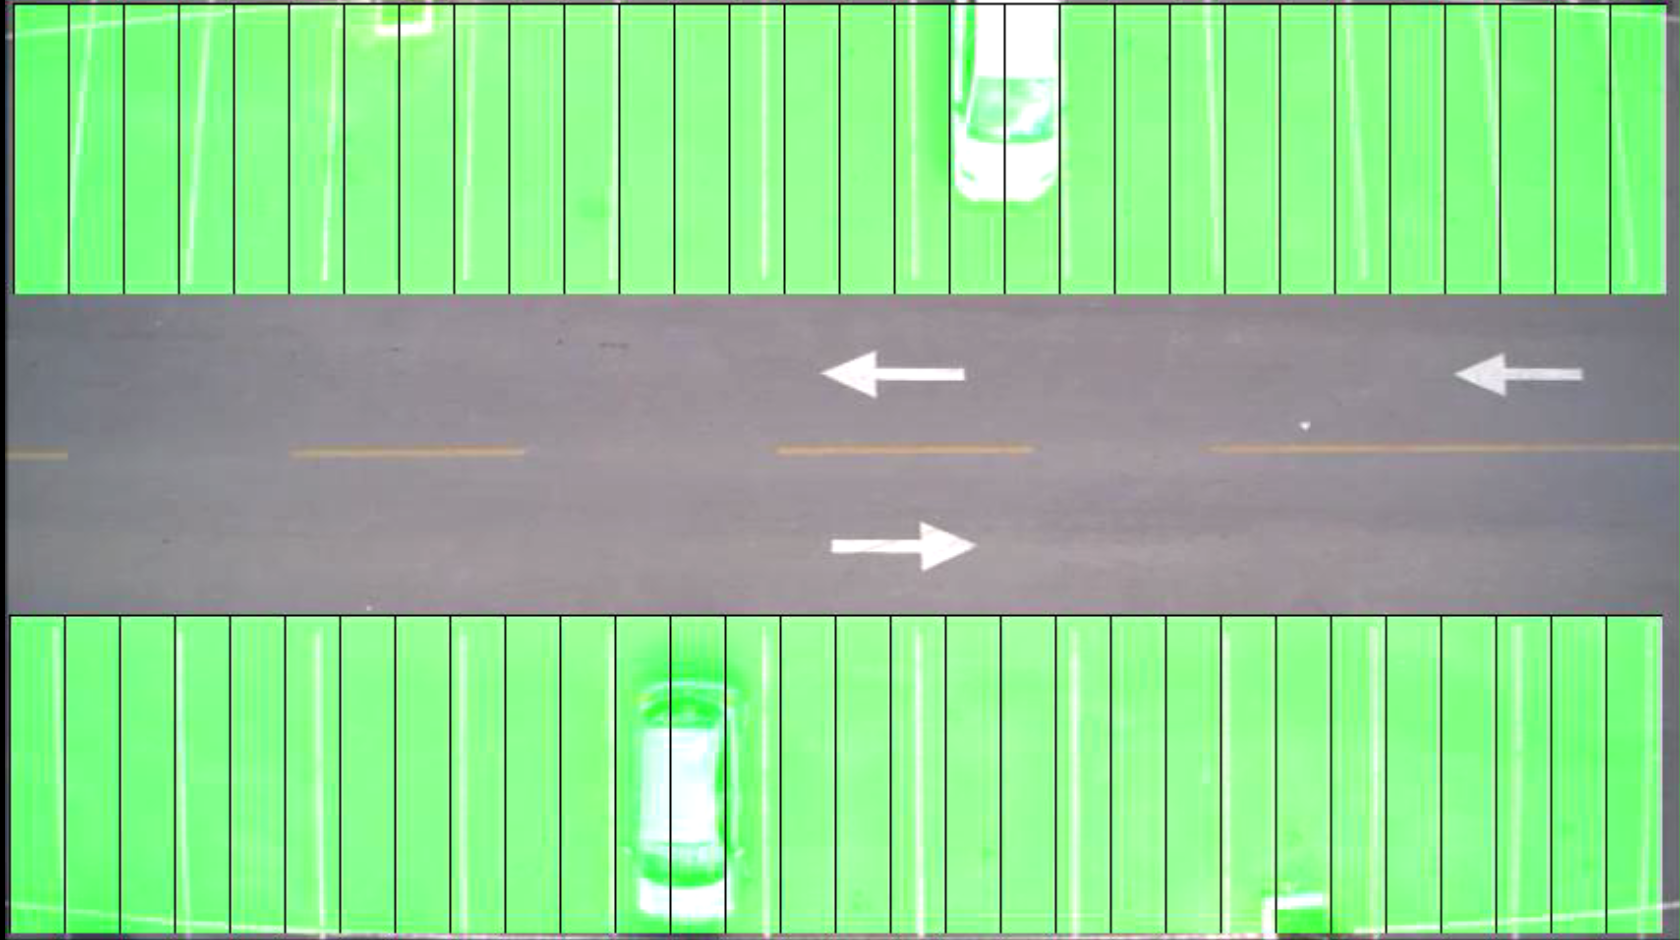
\includegraphics[width=.8\linewidth]{Video5Fim}
\caption{}
\end{subfigure}
\centering
\caption{(a) O momento inicial do vídeo 5. (b) O momento final do vídeo 5}%
\label{}%
\end{figure}

\begin{center}
\begin{tabular}{|c||c|}
\hline
\multicolumn{2}{|c|}{Observador F}  \\ \hline \hline
Tempo(s) & Acontecimento \\ \hline
0 & ROI 1: Seções 15,16,18 e 19 ocupadas. \\
 & ROI 2: Seções 12 e 13 ocupadas. \\ \hline
3 & ROI 1: Seções 15 e 16 liberadas. \\
\hline
\end{tabular}
\end{center}

\begin{center}
\begin{tabular}{|c||c|}
\hline
\multicolumn{2}{|c|}{Observador P}  \\ \hline \hline
Tempo(s) & Acontecimento \\ \hline
0 & ROI 1: Seções 15,16,18 e 19 ocupadas. \\
 & ROI 2: Seções 12,13 e 14 ocupadas. \\ \hline
4 & ROI 1: Seções 15 e 16 liberadas. \\
\hline
\end{tabular}
\end{center}

\begin{center}
\begin{tabular}{|c||c|}
\hline
\multicolumn{2}{|c|}{Observador M}  \\ \hline \hline
Tempo(s) & Acontecimento \\ \hline
0 & ROI 1: Seções 15,16,18 e 19 ocupadas. \\
 & ROI 2: Seções 12,13 e 14 ocupadas. \\ \hline
3 & ROI 1: Seções 15 e 16 liberadas. \\
\hline
\end{tabular}
\end{center}

\begin{center}
\begin{tabular}{|c||c|}
\hline
\multicolumn{2}{|c|}{Programa}  \\ \hline \hline
Tempo(s) & Acontecimento \\ \hline
0 & ROI 1: Seções 15,16,18 e 19 ocupadas. \\
 & ROI 2: Seções 12 e 13 ocupadas. \\ \hline
1 & ROI 1: Seção 17 ocupada. \\ \hline
3 & ROI 1: Seções 15 e 16 liberadas. \\ \hline
4 & ROI 1: Seção 17 liberada. \\
\hline
\end{tabular}
\end{center}

\begin{center}
\begin{tabular}{|c||c||c|}
\hline
Observador & Acertos & Taxa de acertos \\ \hline
F & 597 & 99,50\% \\  \hline
P & 585 & 97,50\% \\ \hline
M & 587 & 97,83\% \\ \hline
Média & 1757 & 97,61\% \\
\hline
\end{tabular}
\end{center}

Um caso de testes simples, onde os erros ocorreram principalmente por causa da natureza subjetiva do que configura uma seção ocupada. O programa classifica a seção $17$ como ocupada e os observadores não. Por outro lado, dois dos observadores acharam que a seção $14$ da ROI $2$ estava ocupada, descordando do programa.

\subsection{Vídeo 6}

Neste vídeo o veículo amarelo entra na cena pela parte inferior da tela. O veículo branco desocupa sua vaga e sai da tela pelo lado esquerdo. O vídeo tem $13s$ totalizando $780$ acertos possíveis.

\begin{figure}[!h]
\centering
\begin{subfigure}{.5\textwidth}
\centering
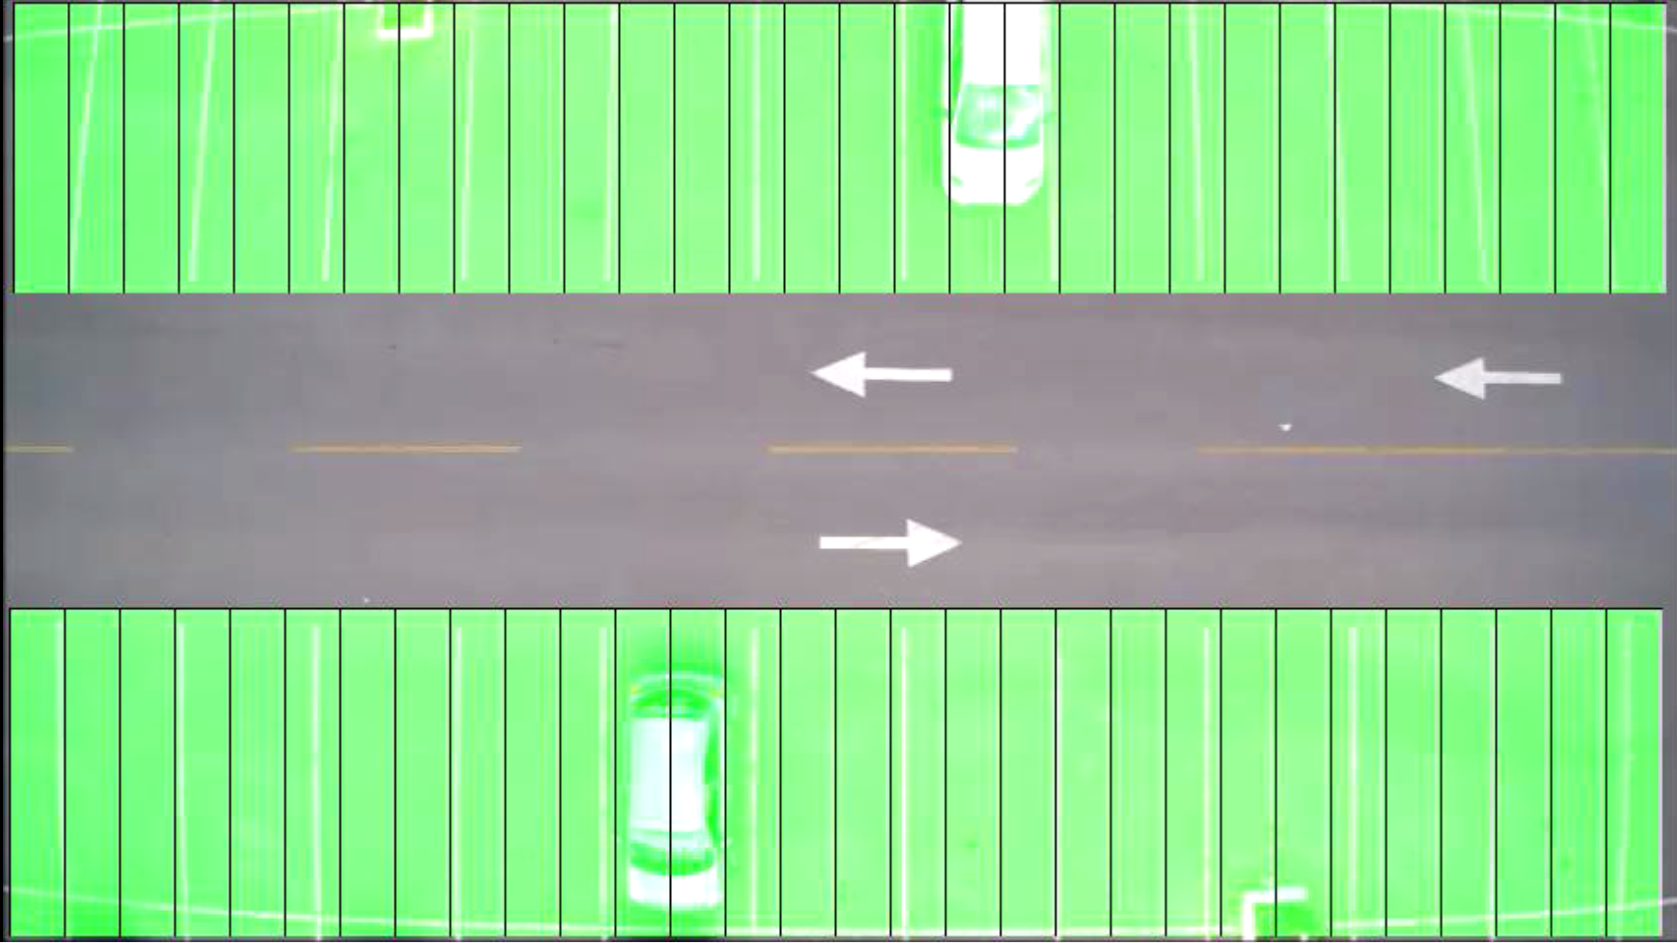
\includegraphics[width=.8\linewidth]{Video6Inicio}
\caption{}
\end{subfigure}\
\begin{subfigure}{.5\textwidth}
\centering
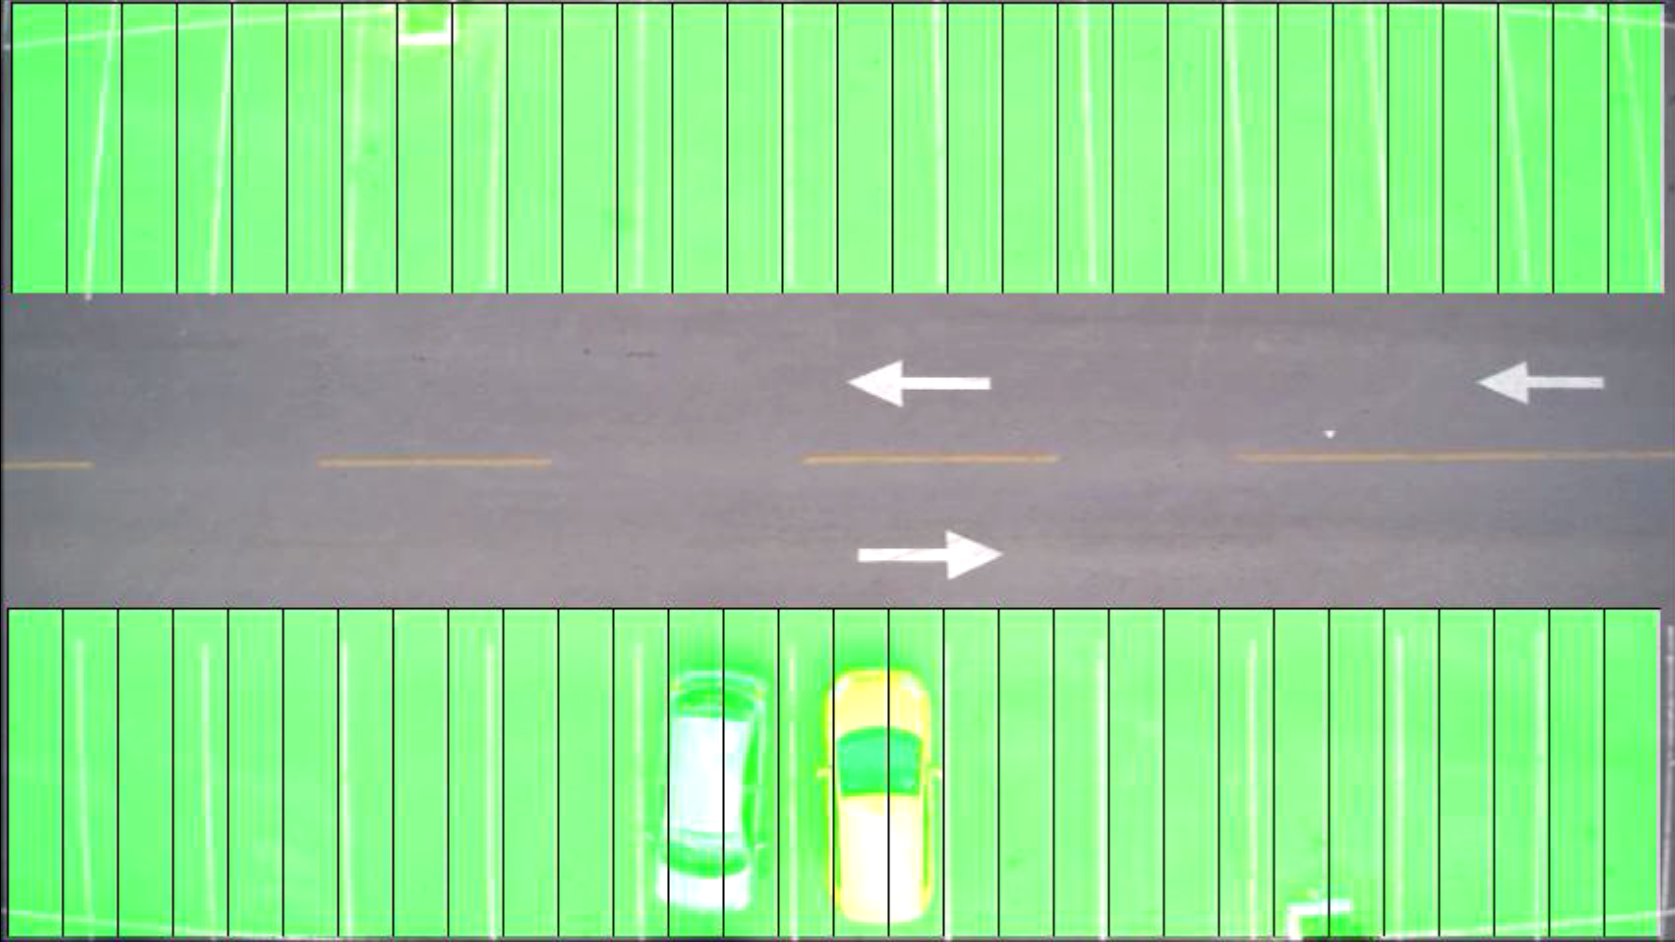
\includegraphics[width=.8\linewidth]{Video6Fim}
\caption{}
\end{subfigure}
\centering
\caption{(a) O momento inicial do vídeo 6. (b) O momento final do vídeo 6.}%
\label{}%
\end{figure}

\begin{center}
\begin{tabular}{|c||c|}
\hline
\multicolumn{2}{|c|}{Observador F}  \\ \hline \hline
Tempo(s) & Acontecimento \\ \hline
0 & ROI 1: Seções 18 e 19 ocupadas. \\
 & ROI 2: Seções 12 e 13 ocupadas. \\ \hline
5 & ROI 2: Seções 14 e 15 ocupadas. \\ \hline
8 & ROI 1:Seçoes 18 e 19 liberadas. \\
\hline
\end{tabular}
\end{center}

\begin{center}
\begin{tabular}{|c||c|}
\hline
\multicolumn{2}{|c|}{Observador P}  \\ \hline \hline
Tempo(s) & Acontecimento \\ \hline
0 & ROI 1: Seções 18 e 19 ocupadas. \\
 & ROI 2: Seções 12 e 13 ocupadas. \\ \hline
5 & ROI 1: Seções 15,16 e 17 ocupadas. \\ \hline
9 & ROI 2: Seções 18 e 19 liberadas. \\
\hline
\end{tabular}
\end{center}

\begin{center}
\begin{tabular}{|c||c|}
\hline
\multicolumn{2}{|c|}{Observador M}  \\ \hline \hline
Tempo(s) & Acontecimento \\ \hline
0 & ROI 1: Seções 18 e 19 ocupadas. \\
 & ROI 2: Seções 12 e 13 ocupadas. \\ \hline
4 & ROI 1: Seções 15,16 e 17 ocupadas. \\ \hline
8 & ROI 2: Seções 18,19 liberadas.\\
\hline
\end{tabular}
\end{center}

\begin{center}
\begin{tabular}{|c||c|}
\hline
\multicolumn{2}{|c|}{Programa}  \\ \hline \hline
Tempo(s) & Acontecimento \\ \hline
0 & ROI 1: Seções 18 e 19 ocupadas. \\
 & ROI 2: Seções 12 e 13 ocupadas. \\ \hline
5 & ROI 2: Seções 15 e 16 ocupadas. \\ \hline
7 & ROI 2: Seção 17 ocupada. \\ \hline
11 & ROI 1: Seções 18 e 19 liberadas. \\
\hline
\end{tabular}
\end{center}

\begin{center}
\begin{tabular}{|c||c||c|}
\hline
Observador & Acertos & Taxa de acertos \\ \hline
F & 752 & 96,40\% \\  \hline
P & 774 & 99,23\% \\ \hline
M & 767 & 98,33\% \\ \hline
Média & 764,33 & 97,99\% \\
\hline
\end{tabular}
\end{center}

Um caso de testes aonde a avaliação do programa se mantém estável e concorda quase plenamente com a avaliação dos humanos. Os atraso da detecção da liberação das seções $18$ e $19$ da ROI $2$ se deve ao fato de que o movimento do veículo saindo só é considerado finalizado depois que ele sai da tela, o que ocorre alguns momentos depois que os observadores humanos consideraram que ele saiu da vaga.

\subsection{Vídeo 7}

Neste vídeo um dos carros sai da cena pela esquerda. O vídeo tem $17s$ de duração e portanto $1020$ acertos possíveis.

\begin{figure}[!h]
\centering
\begin{subfigure}{.5\textwidth}
\centering
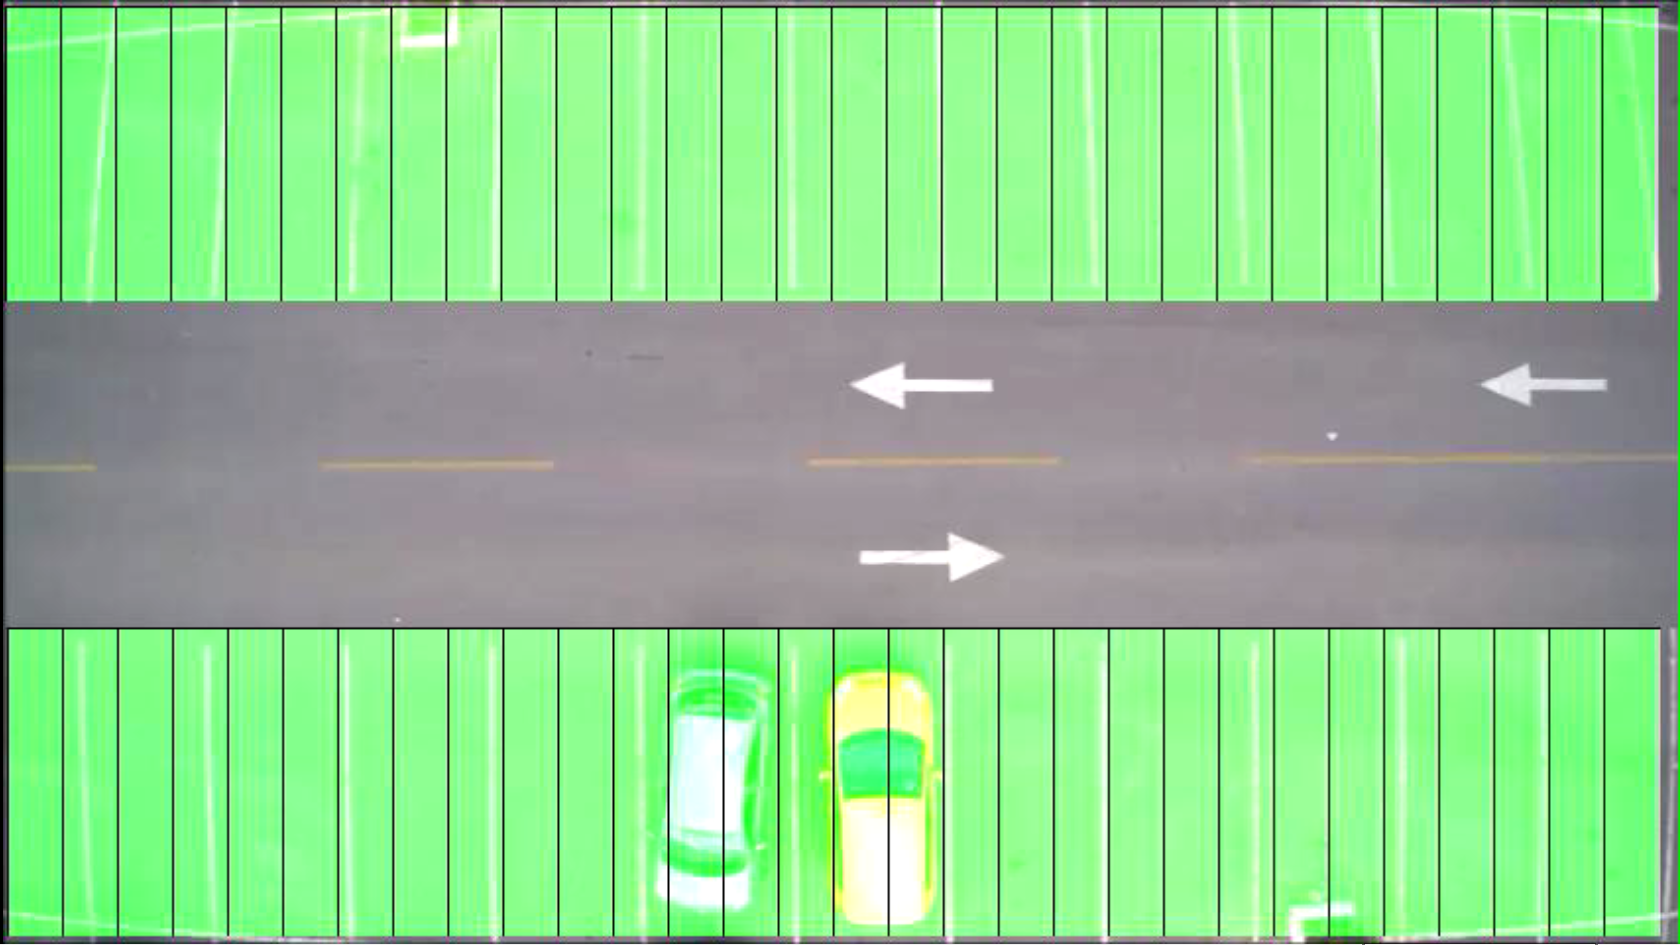
\includegraphics[width=.8\linewidth]{Video7Inicio}
\caption{}
\end{subfigure}\
\begin{subfigure}{.5\textwidth}
\centering
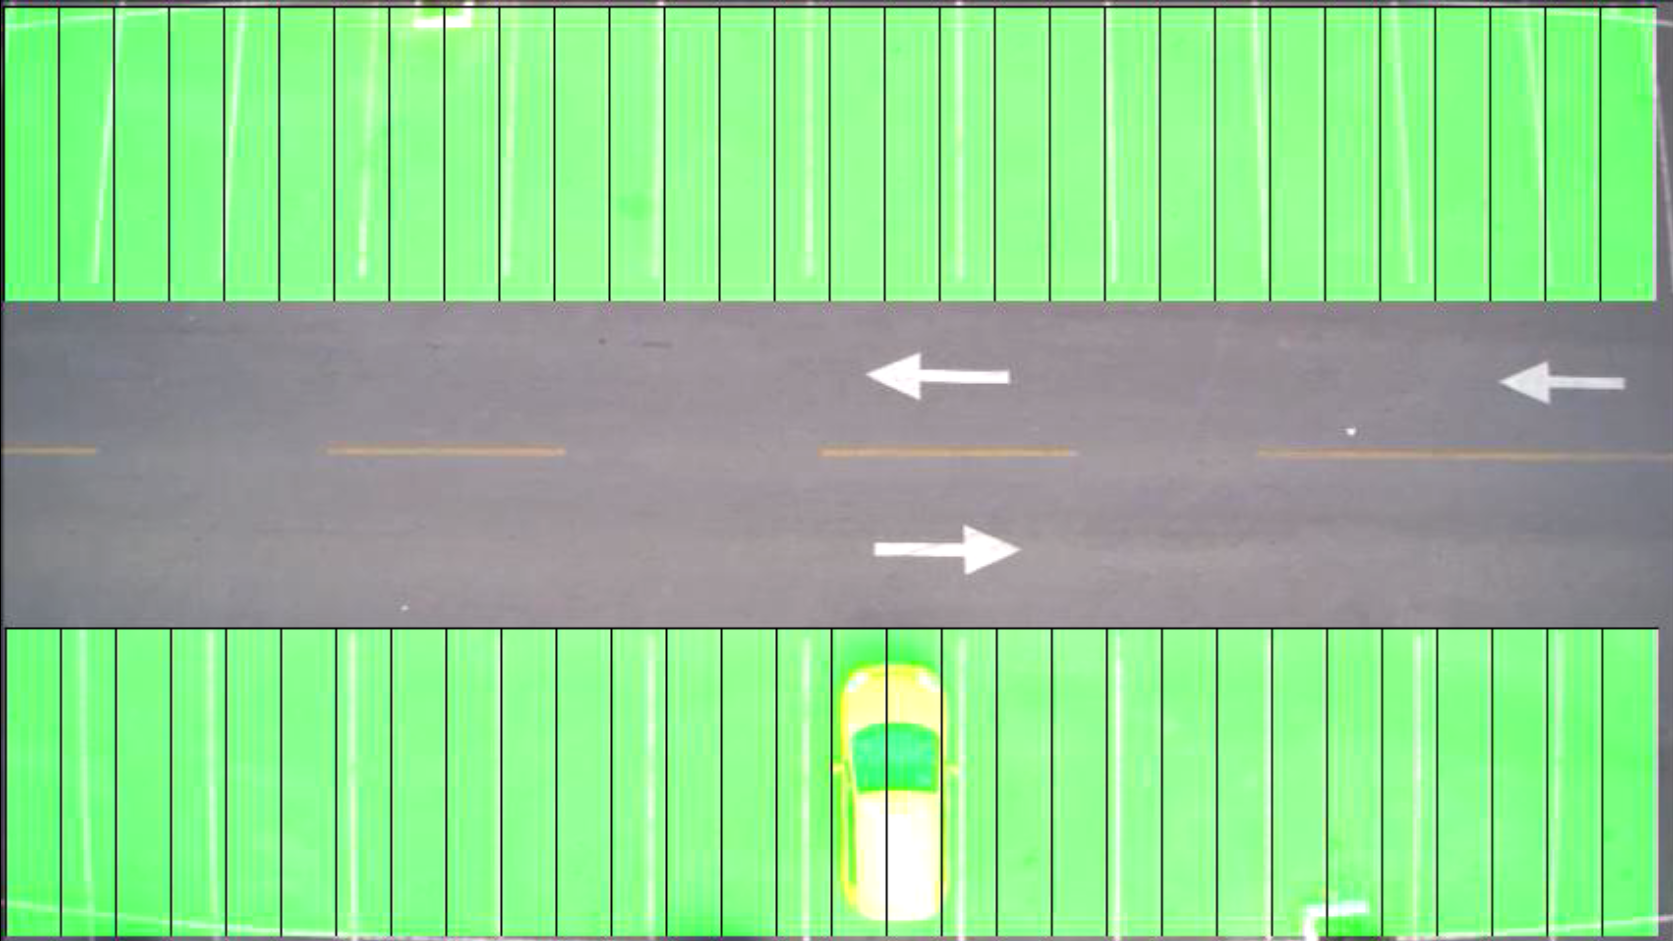
\includegraphics[width=.8\linewidth]{Video7Fim}
\caption{}
\end{subfigure}
\centering
\caption{(a) O momento inicial do vídeo 7. (b) O momento final do vídeo 7.}%
\label{}%
\end{figure}

\begin{center}
\begin{tabular}{|c||c|}
\hline
\multicolumn{2}{|c|}{Observador F}  \\ \hline \hline
Tempo(s) & Acontecimento \\ \hline
0 & ROI 2: Seções 13,14,16 e 17 ocupadas. \\ \hline
4 & ROI 2: Seções 13 e 14 liberadas. \\
\hline
\end{tabular}
\end{center}

\begin{center}
\begin{tabular}{|c||c|}
\hline
\multicolumn{2}{|c|}{Observador P}  \\ \hline \hline
Tempo(s) & Acontecimento \\ \hline
0 & ROI 2: Seções 12,13,14,16 e 17 ocupadas. \\ \hline
6 & ROI 2: Seções 12,13,14 liberadas. \\ 
\hline
\end{tabular}
\end{center}

\begin{center}
\begin{tabular}{|c||c|}
\hline
\multicolumn{2}{|c|}{Observador M}  \\ \hline \hline
Tempo(s) & Acontecimento \\ \hline
0 & ROI 2: Seções 12,13,14,16 e 17 ocupadas. \\ \hline
5 & ROI 2: Seções 12,13,14 liberadas. \\ 
\hline
\end{tabular}
\end{center}

\begin{center}
\begin{tabular}{|c||c|}
\hline
\multicolumn{2}{|c|}{Programa}  \\ \hline \hline
Tempo(s) & Acontecimento \\ \hline
0 & ROI 2: Seções 13,14,16 e 17 ocupadas. \\ \hline
1 & ROI 2: Seção 12 ocupada. \\ \hline
2 & ROI 2: Seção 14 liberada. \\ \hline
5 & ROI 2: Seções 12 e 13 liberadas. \\
\hline
\end{tabular}
\end{center}

\begin{center}
\begin{tabular}{|c||c||c|}
\hline
Observador & Acertos & Taxa de acertos \\ \hline
F & 1013 & 99,31\% \\  \hline
P & 1014 & 99,41\% \\ \hline
M & 1016 & 99,60\% \\ \hline
Média & 1014,33 & 99,44\% \\
\hline
\end{tabular}
\end{center}

O programa concordou com os observadores nesse vídeo, exibindo apenas um leve atraso para a classificação correta da seção $12$ e uma liberação levemente precipitada da seção $14$.

\subsection{Vídeo 8}

No oitavo e último caso de testes, um carro branco passa pela região central da imagem sem estacionar em nenhuma vaga e depois um carro cinza estaciona na região inferior. O vídeo tem $23s$ de duração e $1380$ acertos possíveis.

\begin{figure}[!h]
\centering
\begin{subfigure}{.5\textwidth}
\centering
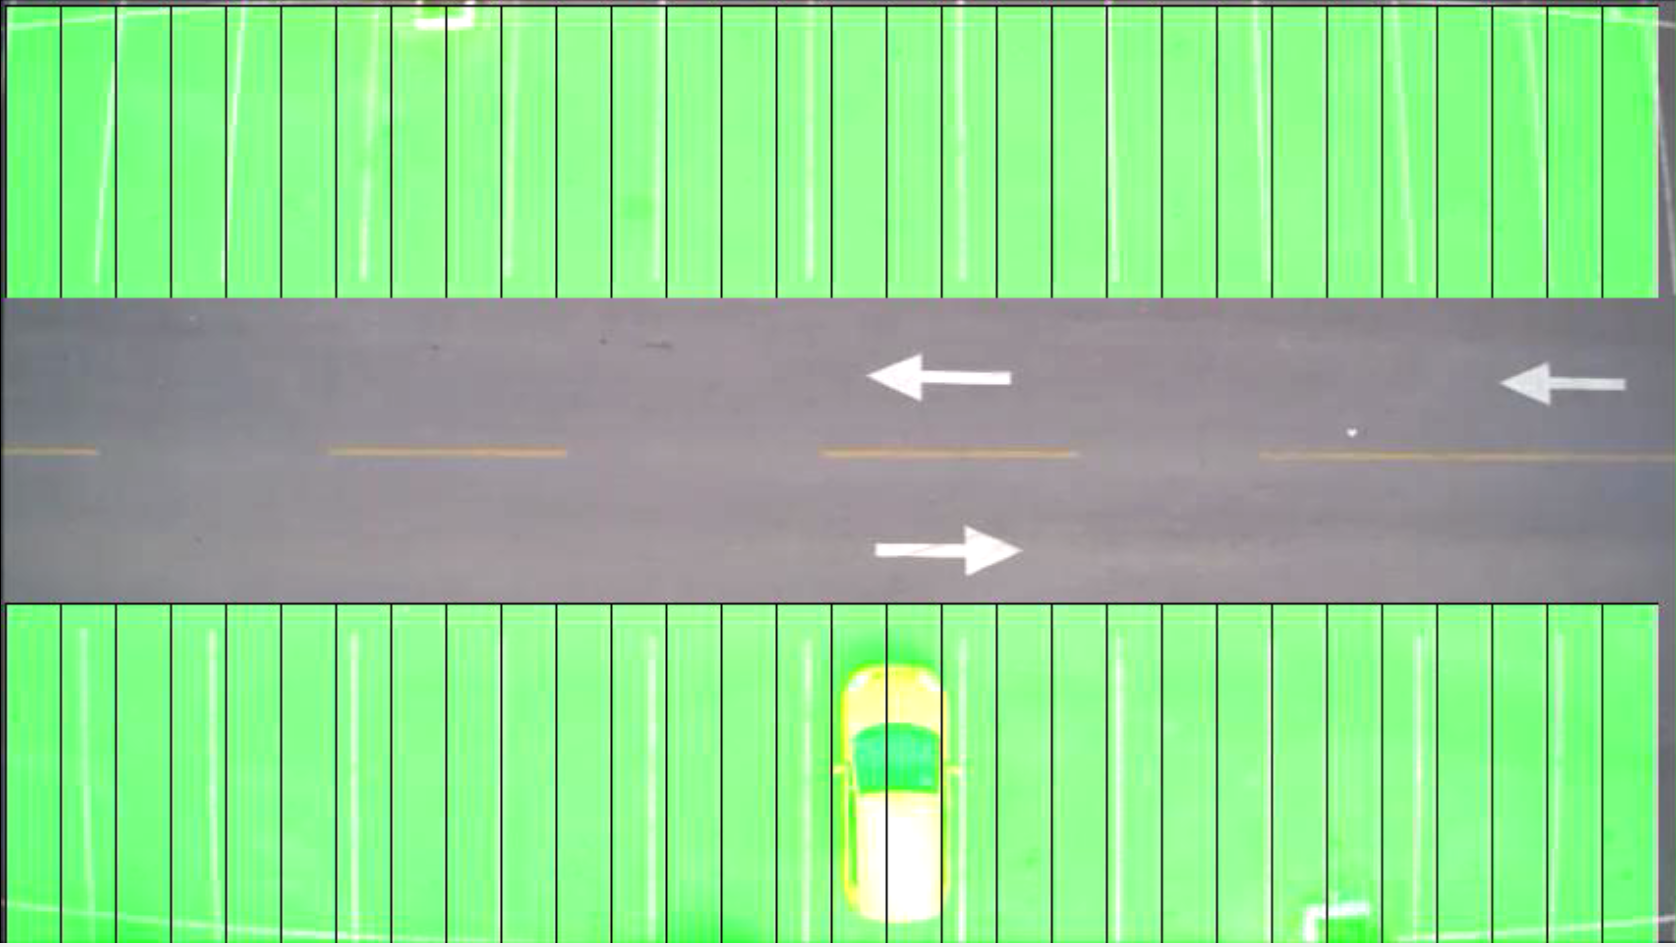
\includegraphics[width=.8\linewidth]{Video8Inicio}
\caption{}
\end{subfigure}\
\begin{subfigure}{.5\textwidth}
\centering
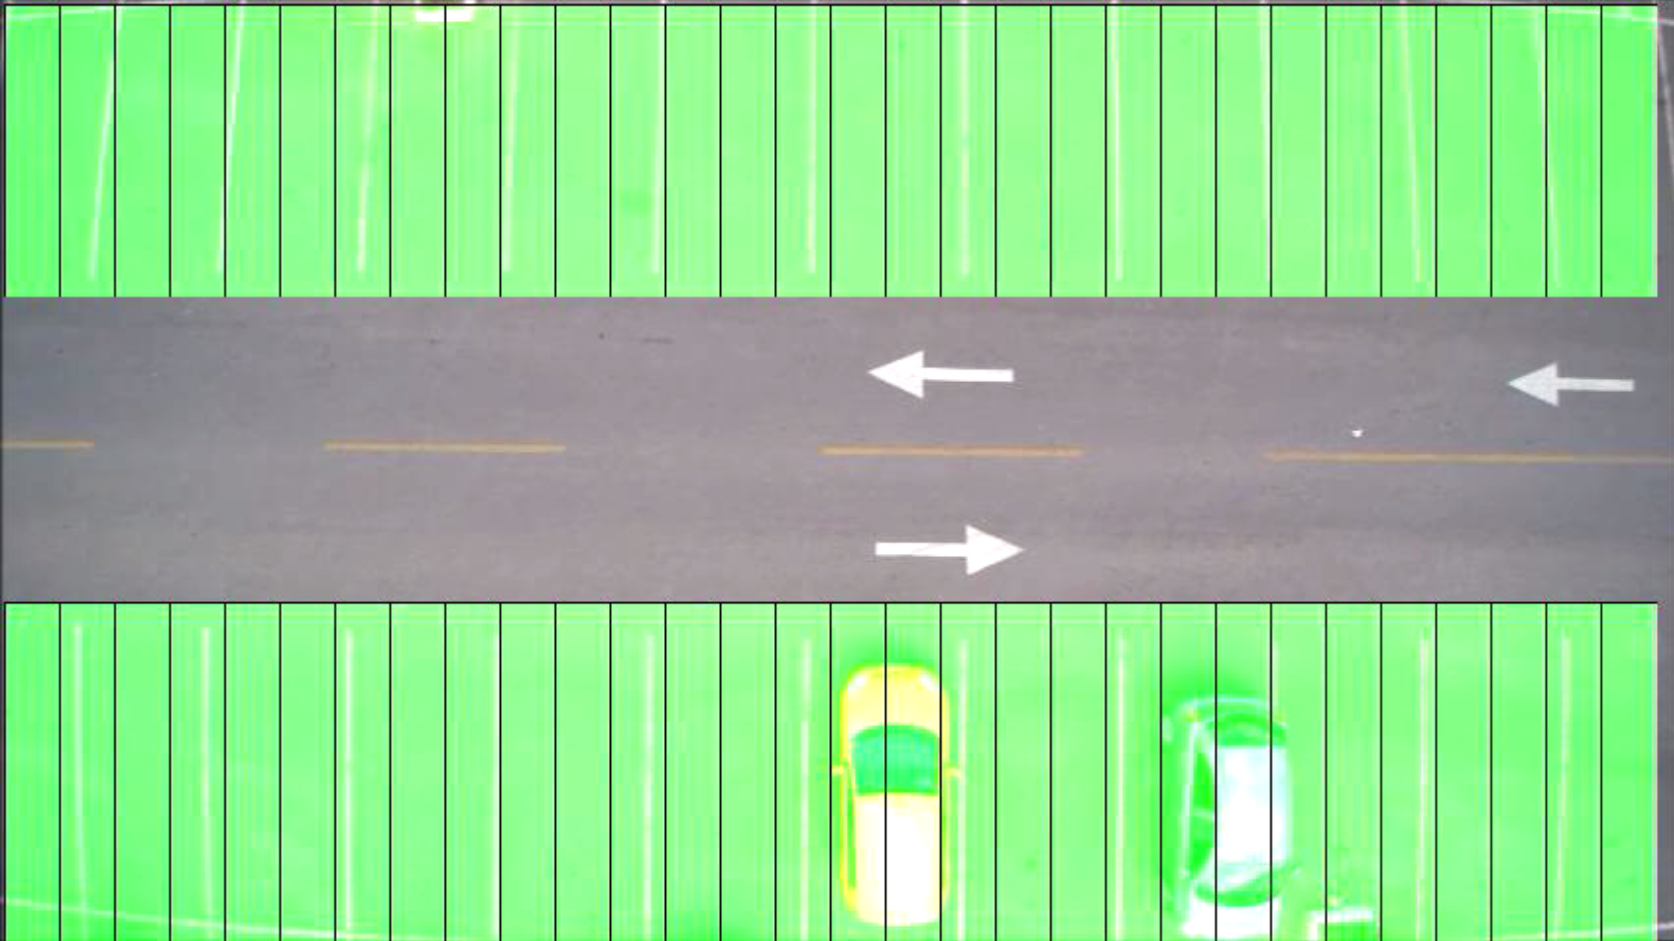
\includegraphics[width=.8\linewidth]{Video8Fim}
\caption{}
\end{subfigure}
\centering
\caption{(a) O momento inicial do vídeo 8. (b) O momento final do vídeo 8.}%
\label{}%
\end{figure}

\begin{center}
\begin{tabular}{|c||c|}
\hline
\multicolumn{2}{|c|}{Observador F}  \\ \hline \hline
Tempo(s) & Acontecimento \\ \hline
0 & ROI 2: Seções 16 e 17 ocupadas. \\ \hline
20 & ROI 2: Seções 22 e 23 ocupadas. \\
\hline
\end{tabular}
\end{center}

\begin{center}
\begin{tabular}{|c||c|}
\hline
\multicolumn{2}{|c|}{Observador P}  \\ \hline \hline
Tempo(s) & Acontecimento \\ \hline
0 & ROI 2: Seções 16 e 17 ocupadas. \\ \hline
20 & ROI 2: Seções 22 , 23 e 24 ocupadas. \\
\hline
\end{tabular}
\end{center}

\begin{center}
\begin{tabular}{|c||c|}
\hline
\multicolumn{2}{|c|}{Observador M}  \\ \hline \hline
Tempo(s) & Acontecimento \\ \hline
0 & ROI 2: Seções 16 e 17 ocupadas. \\ \hline
20 & ROI 2: Seções 22,23 e 24 ocupadas. \\
\hline
\end{tabular}
\end{center}

\begin{center}
\begin{tabular}{|c||c|}
\hline
\multicolumn{2}{|c|}{Programa}  \\ \hline \hline
Tempo(s) & Acontecimento \\ \hline
0 & ROI 2: Seções 16 e 17 ocupadas. \\ \hline
20 & ROI 2: Seções 21,22,23 e 24 ocupadas. \\ \hline
21 & ROI 2: Seção 21 liberada. \\
\hline
\end{tabular}
\end{center}

\begin{center}
\begin{tabular}{|c||c||c|}
\hline
Observador & Acertos & Taxa de acertos \\ \hline
F & 1376 & 99,71\% \\  \hline
P & 1379 & 99,92\% \\ \hline
M & 1379 & 99,92\% \\ \hline
Média & 1378 & 99,85\% \\
\hline
\end{tabular}
\end{center}

O programa avalia as seções de forma quase idêntica aos humanos. Aos $20s$, a classificação que ocorre regularmente determina que que quatro seções estão sendo ocupadas pelo veículo. Um segundo depois porém, quando o movimento do veículo termina, o erro corrige e o programa volta a acertar completamente.












	\chapter{Conclusão}\label{cap:conclusao}

A tarefa de se encontrar vagas em estacionamentos tem se tornado cada vez mais difícil com o aumento da frota de veículos das grandes cidades. Essa busca por um espaço livre para estacionar o carro pode durar muito tempo, criando gastos que se acumulam até valores altíssimos.

Buscando minimizar estes problemas, diversos sistemas de mapeamento de estacionamento e detecção de vagas livres foram desenvolvidos. Algumas soluções são implementadas nos próprios veículos \cite{schmid2011parking}, mas as mais interessantes para uma solução geral do problema são aquelas que detectam a quantidade de vagas livres em uma região do estacionamento e disponibilizam essa informação para todos os seus usuários. Em garagens, sensores de vários tipos podem ser utilizados \cite{kianpisheh2012smart}\cite{wolff2006parking}\cite{lee2008intelligent}, mas estas soluções não são muito adequadas para aplicação em estacionamentos descobertos. 

Para estes casos, uma solução que se mostrou adequada e de fácil implementação foi o uso de câmeras de vídeo e algoritmos de processamento de imagens e visão computacional. Este trabalho apresentou um algoritmo para ser utilizado em um sistema como estes, chamado de \textit{Detector de vagas em estacionamentos abertos}, abreviado como \textit{DVE}. O algoritmo recebe as imagens de câmera de vídeo coloridas montadas em postes de luz e usa uma rede neural artificial combinada com uma técnica de rastreamento dos veículos através do fluxo óptico para mapear e determinar a ocupação das vagas que aparecem na imagem.

O \textit{DVE} é especialmente adequado para estacionamentos descobertos com postes de luz em intervalos de distância regular e com poucas ou nenhuma obstrução visual. Quando testado em vídeos que simulavam a captura de uma câmera instalada em um destes postes, o programa apresentou resultados bastante semelhantes a resultados determinados por um observador humano. Ele apresentou dificuldade em classificar corretamente regiões ocupadas por carros com coloração semelhante a do asfalto quando iluminados de certa maneira. Além disso apresentou a possibilidade de detecção errônea de vagas, o que fazia que fossem acusadas uma ocupação maior do que a real nos vídeos.

Apesar de alguns erros, o \textit{DVE} é resistente a pequenos erros de classificação da rede neural na maioria dos casos e até aos movimentos do equipamento de captura, já que na maioria das vezes continuou detectando o número correto de vagas ocupadas na imagem apesar destes empecilhos.

Por fim, o programa se mostrou promissor e capaz de ajudar de forma simples usuários de estacionamento a encontrarem vagas com mais facilidade. Ainda é necessário, porém, fazer um refinamento do sistema de mapeamento do \textit{DVE}, de forma que ele seja capaz de criar um mapa preciso do estacionamento monitorado e disponibilizar mais informações aos usuários, como tempo médio de espera ou a posição exata das vagas livres. Um outro possíel trabalho futuro é a adaptação do \textit{DVE} para que ele funcione com imagens de câmera em ângulos olíquos ao estacionamento, permitindo uma instalação ainda mais fácil e em estacionamentos mais variados. Já foram feitos experimentos neste sentido usando seções quadradas menores ao invés das seções verticais e a mesma rede neural com resultados premilinares promissores, como exemplificado na figura \ref{fig:preliminares}

\begin{figure}%
\centering
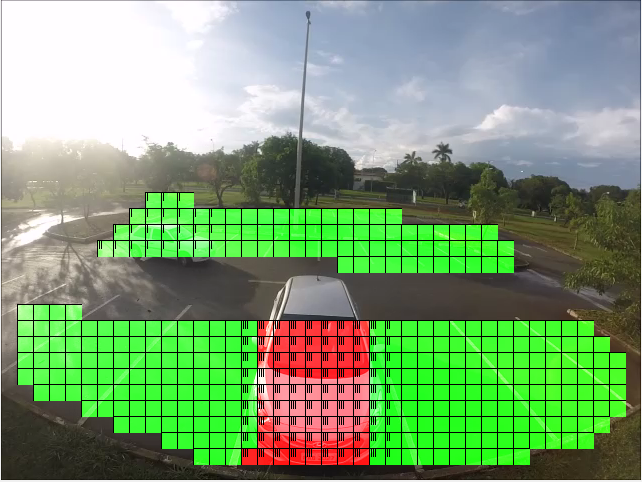
\includegraphics[width=8cm]{preliminar}%
\caption{Resultados preliminares de um possível trabalho futuro.}%
\label{fig:preliminares}%
\centering
\end{figure}










  
  % ...

  \postextual
  \bibliographystyle{unsrt}
  \bibliography{bibliografia}

\end{document}

